\documentclass{smarthepnote}
\usepackage[colorinlistoftodos]{todonotes}
\usepackage{placeins}
%\usepackage{caption,subcaption}
\usepackage{titlesec}

\usepackage{dirtytalk}
\usepackage{siunitx}
\usepackage{subcaption}

\title{Summary of the trigger systems of the Large Hadron Collider experiments ALICE, ATLAS, CMS and LHCb}
\author{The SMARTHEP Network}
\date{\today}

% Here is the information that will be entered in the title page
\DocAuthors{V.~Gligorov \\ C.~Doglioni \\ the SMARTHEP network}
\DocEditors{ L. Bozianu \\ S. Cella \\ C. E. Cocha Toapaxi \\ K. Endrup Iversen (*) \\ P. Inkaew \\ D. Magdalinski \\ D. J. Wilson-Edwards (*)}
\DocCoordinators{J. Albrecht \\ L. Calefice \\ J. A. Gooding \\ A. Sopasakis }
\DeliverableNo{6.1}
\draftversion{1.2}

\def\thickhline{\noalign{\hrule height1.2pt}}

\usepackage{lineno}
\linenumbers

\begin{document}
\maketitle

\begin{abstract}
%This white paper from the SMARTHEP Network reviews the current status of trigger systems employed at the Large Hadron Collider (LHC). The principles of triggering in the current state-of-the-art are discussed and illustrated with recent and ongoing developments from the ALICE, ATLAS, CMS and LHCb collaborations. This review places particular emphasis on real-time data processing approaches and techniques.

In modern High Energy Physics (HEP) experiments, triggers perform the important task of selecting, in real time, the data to be recorded and saved for physics analyses. As a a result, trigger strategies play a key role in extracting relevant information from the vast streams of data produced at facilities like the Large Hadron Collider (LHC). As the energy and luminosity of the collisions increase, these strategies must be upgraded and maintained to suit the experimental needs. This white paper from the SMARTHEP Network presents a high-level overview and reviews recent developments of triggering practices employed at the LHC. Particular emphasis is placed on real-time data processing approaches and techniques. The general trigger principles applied at a modern HEP experiment are highlighted, with specific reference to the current trigger state-of-the-art within the ALICE, ATLAS, CMS and LHCb collaborations. Furthermore, a brief synopsis of the new trigger paradigm required by the upcoming high-luminosity upgrade of the LHC is provided. 

\textit{As of 31/01/2024, this draft has not yet undergone review from experts from the LHC collaborations. Note also that this white paper is not meant to provide an exhaustive review or substitute documentation and papers from the collaborations themselves, but rather offer general considerations and examples from the literature that are relevant to the SMARTHEP  network.} 

%the application of machine learning techniques for real-time analysis (RTA) of collision events at the Large Hadron Collider (LHC). It discusses the crucial role of RTA in addressing the data-processing challenges faced by LHC experiments and how modern ML techniques are helping to overcome them. First, we provide some insights into selecting the most suitable ML algorithms and adapting them to the real- time environment using software techniques and hardware accelerators. Then, we review a small selection of current and future uses of machine learning for RTA that are of particular interest to the SMARTHEP network. We continue by emphasizing the importance of collaborations between the high-energy physics community and industry in tackling these challenges and we showcase the mutual benefits that can be achieved. 
%The white paper is not meant to provide an exhaustive review, but rather some general considerations and a limited number of relevant examples from the literature that are relevant to the SMARTHEP innovative training network

%This document is a draft of the trigger whitepaper written by the ESRs that is going to be circulated within the SMARTHEP network. Parts of it may be made public at a later stage. It is intended to serve as an exercise for the SMARTHEP ESRs to learn more about the trigger systems of different experiments (since many ESRs chose to write about the trigger systems of experiments that they are not members of). 

\end{abstract}

% Make the review table at the bottom of the title page
\vfill
\makereviewtable
\clearpage

% Short documentes dont always need a Table of Content / Figures / Tables, so comment out what is not needed
\begingroup
\color{black}
%\tableofcontents
%\listoffigures
%\listoftables
\endgroup
\pagebreak

%\section{Introduction}
%Its always good to have an introduction, if only to have an example for a section. And here is an example for a reference from the bibtex file (see \cite{einstein}). Its also pretty easy to reference figures (see Figure \ref{fig:examplecernlogo}). \\
%\begin{figure}[ht]
%\centering
%
\includegraphics[width=0.5\textwidth]{images/cernlogo.eps}
%\caption{\label{fig:examplecernlogo} Example of how to include a figure. This works with all sorts of formats, eps, pdf, png.}
%\end{figure}

% this will prevent float objects like figures to be moved past this point in the document.
%\FloatBarrier


%You also have the option of using colored text, for example \color{blue} this part in blue,  \color{red} this part in red  \color{green} and this part in green, before \color{black} going back to black.  

%\begin{enumerate}
%\item Everyone loves an enumerated list.
%\item If you prefer bulleted lists, see below.
%\end{enumerate}

%Of course there are always use cases for list with enumerations, and lists with bullets only, which is why it is useful to have examples of both.

%\begin{itemize}
%    \item Everyone loves a bulleted list.
%    \item If you prefer an enumerated list, see above.
%\end{itemize}

%\section{The first section after the introduction}
%Since an example of a ToC is not much fun with only one section, lets make another one and throw in some subsections as well.


%\subsection{The first sub-section}
%How about structuring the document into more subsections.

%\subsection{The second sub-section}
%Tables are just as easy as figures to construct and reference, for example this one here (see Table \ref{tab:exampletable}).

%\begin{table}[h]
%\begin{center}
%\begin{tabular}{ |c|c|c|p{0.1\textwidth}| } 
%    \hline
%    \rowcolor{lightgray} 
%    col1 & col2 & col3 & col4\\
%    \hline
%    \multirow{3}{4em}{Multiple row} & cell2 & cell3 & cell4 \\ 
%    \cline{3-4}
%    & cell5 & \multicolumn{2}{c|}{cell6 and cell7} \\
%    \cline{3-4}
%    & cell8 & cell9 & cell10 \\ 
%    \hline
%    cell11 & cell12 & cell13 & cell14 \\ 
%    \hline
%    \multicolumn{4}{|c|}{ Multicolumn} \\
%    \hline
%\end{tabular}
%\end{center}
%\caption{A table is as happy about a caption as a figure.}
%\label{tab:exampletable}
%\end{table}

% 25 
% 50 


\section{Introduction}

%Intro

The Large Hadron Collider (LHC) was designed to operate at the highest possible energy and luminosity~\cite{CERN:lhc-design-report} to enable precise measurements of the fundamental components of matter and their interaction, and to seek new physics phenomena. 
In the latest LHC data-taking period, Run 3, protons are accelerated to an energy of \SI{6.8}{\tera\electronvolt}, grouped into bunches in opposing beams which cross one another every \SI{25}{\nano\second}~\cite{CERN:lhc-run3-operation}. 
Capturing the details of proton-proton ($pp$) collisions at a rate of \SI{40}{\mega\hertz} introduces an immense data challenge, in which recording collisions in full detail at a typical LHC experiment would require transferring and writing data at up to ${\sim}\SI{40}{\tera\byte\per\second}$. 
To effectively handle this data flow, High Energy Physics (HEP) experiments employ trigger and data acquisition systems, designed to perform detector data readout, event-building, selection, etc in near-real time, reducing the throughput to a manageable level. Typically, $\mathcal{O}\left(\SI{1}{\giga\byte\per\second}\right)$ of data useful to the physics goals of an experiment is written to permanent storage.

Each LHC experiment discussed in this paper — ALICE, ATLAS, CMS and LHCb — has undertaken considerable research and development in terms of triggers and data acquisition (TDAQ), and their most recent reviews can be found in Refs.~\cite{alice-performance-paper-run1, ATLASTriggerRun3, CMS:run3-detector, LHCb:upgrade_trigger_TDR}.

Developments in computational resources (e.g., the adoption of hybrid architectures) and data processing approaches (e.g., real-time and parallelised software frameworks) have enabled more advanced trigger systems to be developed in recent years~\cite{GPUs-for-hep}. These trigger systems are capable of performing real-time calibration, high-level monitoring, etc. ALICE and LHCb performed significant upgrades to their trigger systems ahead of Run~3 of the LHC (2022-2025)~\cite{alice-upgrade, LHCb:2023hlw}, with ATLAS and CMS planning upgrades of similar scales ahead of the High-Luminosity LHC (HL-LHC) operational period (2029-2040s)~\cite{ATLAS:upgrade-scoping, CMS:upgrade-hllhc}.
In this paper, the current trigger state-of-the art is reviewed, predominantly within the context of Run~3.

% Overview of trigger strategies
% Model detector, what does a non-specific trigger look like?
\subsection{Principles of triggering in High Energy Physics}

The primary function of a trigger system, as laid out in Figure~\ref{trigger-schema}, is to reduce the data rate to be processed, according to the physics priorities of the  experiment~\cite{Jeitler_2017, Smith2020, Beck_2007}. 
The performance of a trigger system can therefore be optimised according to three quantities: high signal efficiency, high background rejection (or equivalently low background efficiency) and affordable throughput/output bandwidth. 
Furthermore, this performance must be quantifiable (e.g., that trigger efficiencies are calculable), robust and deterministic. 
To satisfy these requirements, triggers are typically designed in a tiered structure: a lower-level (often hardware-based) tier performing initial data reduction and coarse selection; followed by a software-based (high-level) tier performs reconstruction of physics objects upon which further selections of events is performed. 
This is not the case for all LHC experiments: LHCb does not employ a lower-level hardware trigger in Run~3~\cite{LHCb:upgrade_trigger_TDR} and the ALICE lower-level trigger does not apply selection~\cite{alice-trigger-run3}.


\begin{figure}[!ht]
    \centering
    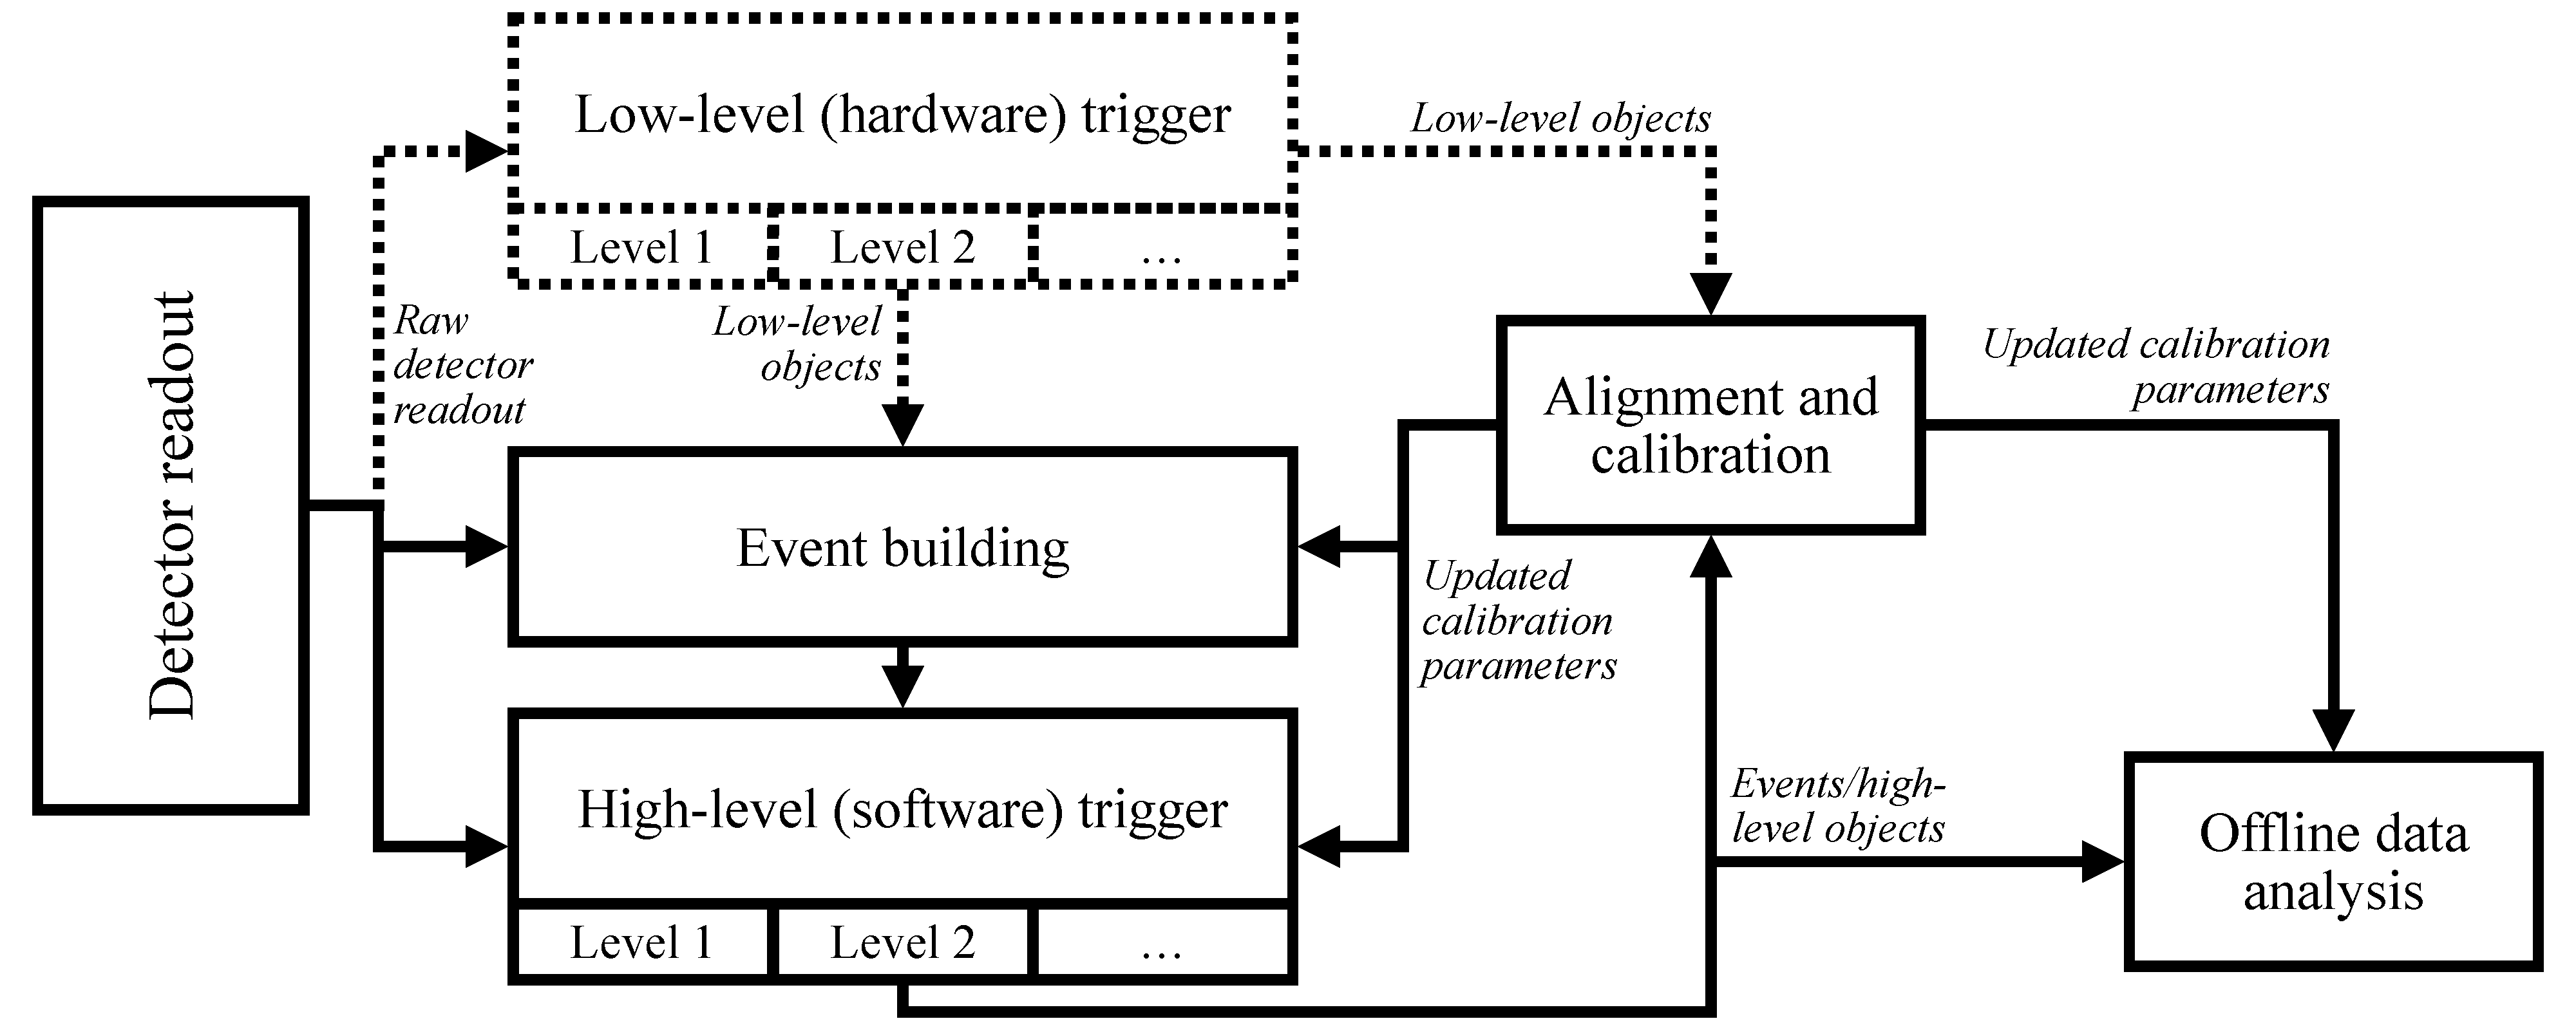
\includegraphics[width=\linewidth]{images/trigger_schematic.pdf}
    \caption[A sketch of a trigger system for a  HEP experiment in the current paradigm. Raw data is read out from each subdetector. A low-level (hardware) trigger is typically employed to synchronise readout and apply initial selection/compression algorithms. A high-level (software) trigger makes further selections on reconstructed objects of increasing accuracy, which are then saved for offline analysis. Alignment and calibration are often performed alongside the high-level trigger to inform the reconstruction algorithms required for detailed selections.]{A generalised schematic of a trigger system for an HEP experiment in the current paradigm. Raw data is read out from each subdetector. A lower-level (hardware) trigger is typically employed to synchronise readout and apply initial selection/compression algorithms. Low-level trigger information and detector readout/reconstructed objects are combined in an event building stage. A high-level (software) trigger makes further selections on reconstructed objects of increasing accuracy, which are then saved for offline analysis. Alignment and calibration are often performed alongside the high-level trigger to inform the reconstruction algorithms required for detailed selections.}
    \label{trigger-schema}
\end{figure}


A lower-level trigger must operate at a rate sufficiently close to the collision rate, and thus must have a minimal dead time between operations. 
The lower-level trigger operates in a staged configuration, increasing latency with each stage to enable more detailed (and thus slower) operations to be performed on the data. 
They are often implemented in custom high-speed electronics to perform operations meeting the latency requirements. 
The data processed by the low-level trigger, typically reduced in rate by a factor $\mathcal{O}\left(100\right)$, is then passed to the high-level trigger for more detailed processing.

Higher-level triggers perform more complex and computationally intensive tasks such as event reconstruction and calibration. 
To ensure that such tasks can be performed at the low-level trigger output rate, the high-level trigger can be separated into two tiers, with the first performing coarse reconstruction and initial selections requiring simpler reconstructed objects (e.g., tracks), and the second performing a detailed reconstruction for more complex selections. 
High-level triggers typically are implemented in computing farm, making use of parallel computing approaches or hybrid computing architectures to efficiently perform tasks within the available computing resources.

The implementations of such systems in each of the major LHC experiments are introduced in the following sections. 

%It is difficult to satisfy both the high efficiencies and high background rejection physics requirements, as well as the very small trigger latency to reduce dead time. Multi-trigger systems are usually introduced. The Level-1 (L1) Trigger is a hardware trigger, comprised of custom high-speed electronics, which makes decisions based off of coarsely reconstructed subset of information from the detector. The L1 trigger renders a selection decision every bunch crossing, with high signal efficiency and comparatively lower background rejection. The data harvested from the L1 trigger is typically more than experiment infrastructure can handle for permanent storage and offline data analysis. Therefore, more sophisticated software Higher Level Triggers (HLT) are usually implemented to further reduce the rate, using full-precision and finer granularity detector information. The maximum allowable acceptance rate L1 trigger is constrained by the detector read out, the speed of at which the HLT performs the more refined selection, and the rate at which the Data AcQuisition (DAQ) system can retrieve the data for permanent storage.  

%The DAQ bandwidth, which is determined by the available storage capabilities and computing power, is related to the maximum allowable trigger rate $R_{\mathrm{trigger}} ^ {max}$ as follows:

\subsection{Trigger systems of the ATLAS and CMS experiments}

The two general-purpose LHC experiments, ATLAS and CMS, have similar, broad physics programmes~\cite{ATLASMachine,collaboration2008cms}. In Run~3, these programmes include searches for new physics: indirectly, by probing the nature of known particles (e.g.,  the Higgs boson~\cite{snowmass-higgs}) at the precision frontier, and directly (e.g.,  through searches for dark matter candidates~\cite{snowmass-darkmatter}). Both experiments consist of concentric layered subdetectors; namely inner detectors for charged particle tracking, calorimeters for measurement of hadron/electromagnetically interacting particle energies and positions, and muon spectrometers for the identification and precise measurement of muons. Due to the wide variety of physics processes probed, the experiments contain a large number of detector channels, resulting in large event sizes of ${\sim}\SI{1}{\mega\byte}$. ATLAS and CMS implement similar two-tier trigger systems with a Level-1 (L1) hardware-based trigger and a software-based high-level trigger (HLT). In Run~2 and Run~3, the triggers of both experiments reduced the initial \SI{40}{\mega\hertz} bunch crossing rate to an L1 acceptance rate of \SI{100}{\kilo\hertz}, reduced further to a final HLT output rate of ${\sim}\SI{1}{\kilo\hertz}$. For average event sizes ranging from ${\sim}\SI{500}{\kilo\byte}$~\cite{ATLASRun3EventBuilder} to ${\sim}\SI{2}{\mega\byte}$~\cite{cmsRun3EventBuilder}, this corresponds to a HLT output bandwidth of $\mathcal{O}\left(\SI{1}{\giga\byte\per\second}\right)$.

\subsection{Trigger system of the LHCb experiment}

The LHCb experiment is a heavy-flavour experiment operating in the forward region, searching for new physics through precision studies of the properties of heavy-flavour decays, in particular CP- and flavour-violation. Following the upgrade of the detector prior to Run~3, the LHCb detector operates as a general-purpose forward detector. The LHCb trigger system was redesigned for Run~3, removing the low-level Level 0 (L0) hardware-based trigger previously employed in Runs 1 and 2. The simplistic cut on $p_{T}$ implemented in the L0 trigger could not discriminate between signal and background for hadronic signals, which would have resulted in a effeciency loss as seen in Fig. \ref{fig:LHCbL0TriggerYield}. As such, the LHCb trigger consists solely of a HLT, split between two stages: HLT1 and HLT2~\cite{Aaij:2019uij}. Following the removal of the L0 trigger, LHCb event readout has increased from \SI{1}{\mega\hertz} to \SI{30}{\mega\hertz}. During Run~2, HLT1 and HLT2 were decoupled to allow HLT1 to run synchronous to data-taking and HLT2 to run asynchronously, enabling  detector calibrations between the steps to improve reconstruction performance to offline quality~\cite{LHCb:Albrecht_2015}. 

\begin{figure}[h!]
    \centering
    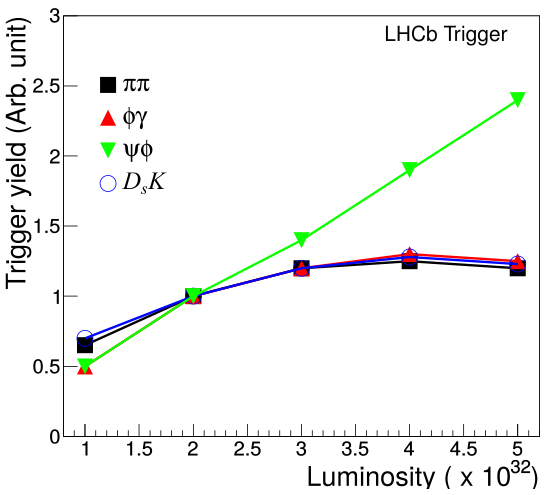
\includegraphics[width=0.55\linewidth]{images/lhcb/LHCb-L0-yield.png}
    \caption{Trigger yield per mode of interest with the Run 2 trigger configuration from Ref.~\cite{LHCb:upgrade-piucci}. Any increase in luminosity from accelerator upgrades is suppressed by the L0 trigger in all modes but $\psi\phi$ (i.e., non-muonic modes).}
    \label{fig:LHCbL0TriggerYield}
\end{figure}

HLT1 was upgraded throughout Run 2 to perform a partial reconstruction of the full detector readout. To achieve this, the reconstruction algorithm was upgraded to be able to run on GPUs hosted on the same event-building servers that host the FPGA cards required to receive data from the detector at 30 MHz~\cite{LHCb_Allen_GPU}. Reconstructed, selected events are propagated to a buffer at an event rate of ${\sim}\SI{1}{\mega\hertz}$. HLT2, implemented as a CPU farm known as the Event Filter Farm (EFF), takes as input the most recent detector alignment and calibration, reconstructing events in full offline quality for detailed selection. This selection reduces the event rate to \SI{100}{\kilo\hertz}, corresponding to an output bandwidth of \SI{10}{\giga\byte\per\second}~\cite{lhcb_hlt2_storage_run3}.

\subsection{Trigger system of the ALICE experiment}
The ALICE experiment is dedicated to the study of heavy-ion collisions at the LHC, with a focus on studies of quantum chromodynamics in energy-dense environments (e.g.,  quark-gluon plasma)~\cite{alice-performance-paper-run1}. To study such environments, ALICE studies p-p, p-Pb and Pb-Pb collisions at frequencies of \SI{1}{\mega\hertz}, \SI{500}{\kilo\hertz} and \SI{50}{\kilo\hertz}, respectively \cite{alice-trigger-run3}. Heavy ion collisions result in a very high multiplicity of particles, with ${\sim}\SI{700}{\mega\byte}$ of raw data per collision event collected by the ALICE experiment \cite{alice-rta-trigger}. The ALICE detector is barrel-shaped, containing concentric particle tracking and identification systems, and a forward muon spectrometer. At the core of the barrel is a Time Projection Chamber (TPC) vital to tracking performance, contributing the majority of the event size (\SI{95.3}{\percent} and \SI{91.1}{\percent} of total data volume in Pb-Pb and p-p collisions, respectively).

The ALICE trigger was upgraded ahead of Run~3 to facilitate continuous readout of subdetectors at collision frequency. The Central Trigger System (CTS), is responsible for the synchronisation of raw detector readout. The CTS transmits aggregated data and trigger signals to the HLT. The HLT then performs event reconstruction, data volume reduction and subdetector calibration, processing data at a maximum rate of \SI{48}{\giga\byte\per\second} to achieve an output throughput of up to \SI{12}{\giga\byte\per\second}~\cite{alice-rta-trigger}.


\section{Acquisition of data}
% Introduce and group ATLAS+CMS+ALICE/LHCb
The first stage of any trigger system involves the readout of detector information (e.g.,  energy deposits in a calorimeter/tracker) and processing of this information. This processing has two main facets: event-building, synchronising information from separate subdetectors to ensure that the corresponding data are correctly associated and the reduction of data volume. The latter is generally accomplished through a combination of basic compression techniques (e.g., zero suppression) and simple selections. These simple selections are commonly performed before readout and event-building, meaning that the information is highly localised to the subdetectors with limited possibilities of combining the information. This is the common task of a low-level trigger. This section covers only ATLAS, CMS and ALICE, since LHCb no longer employs a low-level trigger: detector information is read out continuously by TELL40 readout boards (with compression applied upon readout) and passed to the event builder InfiniBand-based network of HLT1~\cite{LHCb:2023hlw}. The smaller event size and non-hermetic layout(readout cables sit outside detector acceptance) means this change is more achievable for LHCb than ATLAS and CMS.

%Large ATLAS on tiered trig sys, similar structure in CMS, slight difference in ALICE, then tiny LHCb caveat/sentence to be discussed later

%ATLAS+CMS+ALICE
The initial hardware-based L1 triggers of ATLAS~\cite{ATLASRun3Detector} and CMS~\cite{cms2023development} both reduce the rate of data down to a maximum detector read out limit of \SI{100}{\kilo\hertz}, within a latency of \SI{2.5}{\micro\second} at ATLAS and \SI{4}{\micro\second} at CMS. The systems consist of custom ASIC- and FPGA-based\footnote{Algorithm Specific Integrated Chips and Field Programmable Gate Arrays, respectively~\cite{asics-fpgas}.} electronics which use reduced granular information from the calorimeter and muon systems to perform coarse selections. Upon an event passing this selection, the L1 directs the readout hardware of each subdetector to process the surviving data, which is stored in associated local buffers. Information from each subdetector is  then readout, processed and combined within a central readout system where events are assembled. It is buffered until requested by the HLT. The data acquisition (DAQ) systems of both experiments have evolved to use consumer network and computing hardware downstream of custom on-board electronics. This setup simplifies the readout in complexity, maintenance cost and upgrade capabilities. At ATLAS the Front-End LInk eXchange (FELIX)~\cite{ATLAS:FELIX} readout boards, responsible for the interface between commercial and custom hardware, have been partially implemented in Run 3 and will be fully implemented for HL-LHC.


In Run~3, several of the ALICE subdetectors have been upgraded to read out data continuously. The CTS synchronises data, subdividing readout into HeartBeat (HB) frames of approximately 1 LHC orbit period ($\sim\SI{88.92}{\micro\second}$). An HB frame is only kept if all relevant readout units (up to 441 in the entire detector) can be read out. Each HB decision is transmitted asynchronously to the First Level Processor, instructing it on what data to keep in a given HB frame. Whilst many subdetectors (including the TPC) were upgraded to read out data continuously in Run~3, continuous readout is not possible for some subdetectors, e.g.,  the Transition Radiation Detector. Such subdetectors are operated on a triggered basis and are hence excluded from the HB decision calculation, instead using the existing RD12 TTC protocol developed for Run~2 operation. Triggered subdetectors thus operate independently, with triggered data combined with continuous readout data at a later stage~\cite{alice-trigger-run3}.


\section{Reconstruction of event objects}

The reconstruction of events from detector information is a key function of any trigger system; trigger selections typically involve imposing conditions on reconstructed objects including particle tracks and calorimeter clusters. 

In the following, we will focus on examples of reconstruction tasks that are performed \textit{online} within the trigger system of different experiments. 
We denote with \textit{offline} reconstruction tasks those that are performed on objects in events selected by the trigger system at a later stage.  

The complexity and performance requirements of online reconstruction methods can range from fast, lower-level algorithms to full, offline-quality reconstruction of entire events and is determined by the requirements of the given trigger stage. 
It is important for online algorithms to be aligned with (ideally identical to) offline algorithms in terms of inputs, implementation and performance, so that there is a good match between physics objects that inform the event selection and physics objects used for analysis. 
This is also crucial for real-time physics analysis, as discussed in Section \ref{sec:RTA_physics}. 

\subsection{LHCb online tracking algorithms}

In this section we describe the LHCb reconstruction procedure as anexample of the processes involved in reconstructing event objects such as tracks. Similar processes take place in the reconstruction chains of the other LHC experiments with variations due to the specific detector architecture.
% The LHCb reconstruction procedure provides a clear example of the processes involved in reconstructing events and event objects. 

In HLT1, information from the three tracking detectors—Vertex Locator (VELO), Upstream Tracker (UT) and Scintillating Fibre (SciFi) Tracker 
\todo[inline]{Citations for tracking detectors needed}
are used to perform partial event reconstruction in the dedicated CUDA-based software framework Allen~\cite{LHCb_Allen_GPU}. 
\todo[inline]{Need to define partial event reconstruction}
For each sub-detector, many of the following processes must be performed: decoding of input into the global coordinate system; clustering of hits within a detection plane; combination of hits/clusters from different detection layers to form particle trajectories; fitting of track model to track candidates; vertex-finding between tracks.

In the VELO, reconstruction begins with the clustering of hits on each silicon plane, with a bit mask-based clustering algorithm operating in parallel across the local regions of each cluster. Straight-line tracks are then reconstructed, starting with seeds of three hits from consecutive silicon planes, extended to the remaining layers and fit with a simple Kalman filter (discussed further in Section~\ref{sec:Algorithms}). 
Finally, primary vertex (PV) candidates are identified and matched to the tracks. Rather than mapping tracks one-to-one with PV candidates, each track receives a per-candidate weight (corresponding to the likelihood it is associated to each PV candidate) to enable parallel computation. 

UT hits are instead assigned to extrapolated VELO tracks using a minimum momentum cut-off, with the track momentum calculated from the curvature between the straight-line VELO tracks and UT hits.

Tracks passing the VELO and UT are extrapolated to create a search window in the SciFi, where seeds of three hits in different layers are formed. A $\chi^2$ fit is performed on the seeds, and the best seeds are extrapolated to the remainder of the SciFi layers. Since the discrimination power of the three initial hits is limited, several seeds are extrapolated for each UT track, performing additional fits to select the best track per UT track. Hits in the muon systems are matched to extrapolated SciFi tracks according to the track parameters obtained in the previous steps~\cite{LHCb:2023hlw, LHCb_Allen_GPU}.

\todo[inline]{This reads as a description of an offline algorithm, and needs some more considerations or a bottom line that is specific of the reconstruction in trigger.}

\todo[inline]{Not sure how the paragraph below fits in here, consider removing?}
Another class of algorithms that is widely used at LHC experiments is Kalman filters (KFs). KFs are recursive algorithms used for state estimation and data fusion (i.e., combination of information from multiple sensors), with a well-established position as a key reconstruction tool~\cite{kalman-track}, and are particularly well-suited for problems involving dynamic (i.e.,  time-dependent) systems and noisy measurements. KFs combine information from previous state estimates and new measurements to provide an optimal estimate of the current state, taking into account both the dynamics of the system and the uncertainties associated with each measurement~\cite{FRUHWIRTH1987444}. KFs are employed across the major LHC experiments for the tracking of charged particles~\cite{Belikov:2003yr,ATLAS:tracking,CMS:tracking,LHCb_Allen_GPU}

%Central trigger
%Readout->trigger

\subsection{CMS Particle Flow algorithm} \label{sec:Algorithms}

An ever-increasing collection of algorithms for reconstruction of events and constituent objects are developed and adopted by collider physics experiments. One example is Particle Flow (PF)~\cite{sirunyan2017pflowcms} that combines measurements from the various sub-detectors in the ATLAS and CMS sub-detectors to produce particle candidates from the entire event. The general PF process can be briefly summarised as follows: the full detector output is used to describe the global collision event, identifying several basic elements individually and iteratively clustering them together into more complex composite physics objects~\cite{CMS:2020uim,CMS:2018rym,CMS:2014pgm}. The reconstructed physics objects are used to build electrons, muons, tau leptons, photons, jets, missing transverse momentum and other physics objects~\cite{CMS:2018jrd,CMS:2016lmd,CMS:2019ctu}. The physics performance is ameliorated by the combination of measurements from the different sub-detectors which achieve optimal accuracy in different regions of phase space. For example, the best momentum resolution is attained at low transverse momenta in the inner detector tracker and at high transverse momenta in the calorimeter. The composition of the tracks and calorimeter clusters (particle flow objects (PFOs)) are used in jet reconstruction to produce PFjets .

The PF procedure is widely-used in CMS reconstruction in both the trigger and offline analyses. The CMS detector design is well-suited to the use of PF reconstruction: a highly-segmented tracker, fine-grained electromagnetic calorimeter, hermetic hadron calorimeter, strong magnetic field and excellent muon spectrometer provide full, high quality coverage~\cite{sirunyan2017pflowcms}. The ATLAS experiment has expanded its usage of PF in the trigger for Run 3 to include hadronic jet reconstruction. The improvement in resolution is less pronounced in ATLAS due to the excellent energy resolution of the calorimeters and jets produced using only calorimeter clusters, however there is significant improvement in the rejection of pile-up (collisions in addition to the collision of interest occurring within the same detector sensitivity window)~\cite{ATLASTriggerRun3,ATLASJetPFlow}. 

% a widely-used reconstruction procedure in CMS offline analyses, now considered the ``baseline" for object reconstruction in the CMS HLT. The purpose of the PF algorithm is to reconstruct and identify all particles involved in a collision by combining and correlating information from all sub-detectors. The CMS detector design is well-suited to the use of PF reconstruction: a highly-segmented tracker, fine-grained electromagnetic calorimeter, hermetic hadron calorimeter, strong magnetic field and excellent muon spectrometer provide full, high quality coverage~\cite{sirunyan2017pflowcms}. The ATLAS experiment implements PF algorithms offline and partly online. The ATLAS detector gains less from the approach due to its excellent energy resolution in the calorimeters but for low-momentum resolution and pile-up rejection the improvement is substantial~\cite{ATLASTriggerRun3,ATLASJetPFlow}.

\subsection{ML b-jet identification algorithms in ATLAS} \label{sec:Algorithms}

More recently, machine-learning-based algorithms have emerged as options for fast reconstruction. In particular, Graph Neural Networks (GNNs), a class of machine learning models designed to operate on graph-structured data, have seen increasing adoption across the LHC experiments. For example, GNNs are used in the ATLAS Run~3 $b$-jet trigger, where tracks of common vertices are grouped and predictions around jet origin are made~\cite{ATLASTriggerRun3}. 

GNNs propagate information through the nodes and edges of a graph, capturing complex relationships and dependencies within the data. GNNs can learn to perform various tasks, such as node classification, link prediction, and graph classification, for example the cluster of hits and reconstuction of showers in the LHCb calorimeter systems \cite{canudas2022graph}.

\todo[inline]{Need an example of an ALICE algorithm to complete the set of examples.}


\section{Alignment and calibration of detectors}

Accurate alignment and calibration of detectors are crucial to the quality of event reconstruction, ensuring faithful decoding of raw detector information to reconstructible objects. This is particularly important for offline-quality reconstruction, where the final reconstructed objects are later used in physics analysis. Alignment and calibration are typically implemented together %(where alignment often refers to tracking subdetectors and calibration to non-tracking subdetectors, e.g., calorimeters),
performing a minimisation of parameters describing the physical offsets experienced in a given subdetector, e.g., residuals between the expected position of a track and the measured position. Alignment and calibration techniques are also applied online when partial reconstructions and trigger decisions require more accurate knowledge of an object. The real-time approaches of LHCb and ALICE in Run~3 typify this and are thus the focus of this chapter. 
At ATLAS and CMS, the more complex detector nature and the need for the full dataset to obtain sufficiently large calibration samples currently hinders a similar full alignment and calibration strategy in real time.

% LHCb
%\subsection{Real-time detector alignment in LHCb}
To enable the use of real-time alignment and calibration of the LHCb detector the trigger system was designed with a large timing budget between HLT stages, provided by a disk buffer of 30 PB. The online LHCb calibration ensures offline-quality reconstruction, enabling trigger selection with high signal efficiencies. This calibration is typically separated into the alignment of the VELO, UT/SciFi, muon stations and RICH mirrors, and the calibration of the ECAL and RICH. A dedicated data sample\footnote{In addition to triggers which select events for offline analysis at LHCb, dedicated triggers which select events required for alignment and calibration purposes are employed. Events selected by the latter are saved into a dedicated stream described in Section~\ref{sec:data}.} is collected, from which the alignment framework calculates updated alignment constants at regular intervals, i.e., per fill or run, as soon as sufficient data has been collected for precise calculation of the constants.

The alignment constants for the tracking detectors are determined by minimising track reconstruction parameters with respect to the degrees of freedom of each alignable detector element, i.e., translations and rotations in each spatial dimension~\cite{LHCb:wouter-kf}. The UT and SciFi are also aligned using reconstructed tracks traversing the entire tracking system to achieve high track-momentum resolution~\cite{Reiss:2846414}. The ECAL is calibrated by analysing a specific mass distribution in each ECAL cell, providing a mass shift from the known position which can be applied as an adjustment of the photomultiplier tubes after each fill. The RICH is aligned and calibrated on a per-run basis, comparing the distribution of hits and Cherenkov angles to anticipated distributions to generate alignment and calibration constants~\cite{LHCb:RICH_AlignCalib}.
%the $\pi^0\rightarrow \gamma\gamma$ 

% ALICE
%\subsection{Real-time TPC alignment in ALICE}
At ALICE, as a consequence of upgrades for continuous readout in Run~3, the TPC requires real-time calibration to correct for space-charge density distortions which are particularly problematic in high pile-up scenarios. Fluctuations in space-charge distortions vary on a scale of \SI{10}{\milli\second} and need to be corrected for. Average space-charge distortions are corrected with the aid of relevant subdetectors; however, the calibration of average space-charge distortions requires $\mathcal{O}\left(\mathrm{minutes}\right)$ of data collection to form a reliable correction map. Convolutional neural networks (CNNs) are employed to predict the fast-varying fluctuations in space-charge distortion, obtaining a reliable calibration at the fluctuation timescale. The CNN models run on GPUs directly in the HLT farm, resulting in a significant speedup of the TPC calibration.

\section{Handling of data}
\label{sec:data}

Reconstructed detector events are typically complex data objects described by many parameters. The size of events presents a storage challenge as it can become infeasible to write all reconstructed data to memory at the output rate of the high-level trigger. To overcome this challenge, two key strategies are employed to reduce the size of the reconstructed objects. Firstly, the amount of information can be reduced, by selecting only the minimal amount of parameters necessary to sufficiently describe the event to be propagated to storage. Secondly, the object information itself can be compressed, maintaining most or all of the original information while significantly reducing the size of the data being written.

% Streaming
%\subsubsection{Data scouting at ATLAS (TLA) and CMS}
An example of the first approach is the CMS data scouting stream or TLA in ATLAS, wherein events are stored at higher rates with smaller event content - storing simply the online objects, bypassing offline reconstruction entirely. In addition, a parking stream or delayed stream saves event data without running offline reconstruction algorithms, with the intent of processing said events during shutdown periods when computing resources are less constrained. Monitoring and calibration streams are also able to make use of their small event size to store more events, with a typical calibration stream event size of ${\sim}\SI{1.5}{\kilo\byte}$, in comparison to an event with full detector readout at around \SI{2}{\mega\byte}~\cite{cms2023development}. However, the additional information of the latter event model allows a wide range of track reconstruction algorithms to be applied for the identification of b-jets, lepton isolation and the mitigation of pile-up vertices~\cite{mia2014trackingcms,tosi2016trackingcms}. 

\begin{figure}[h!]
    \centering
    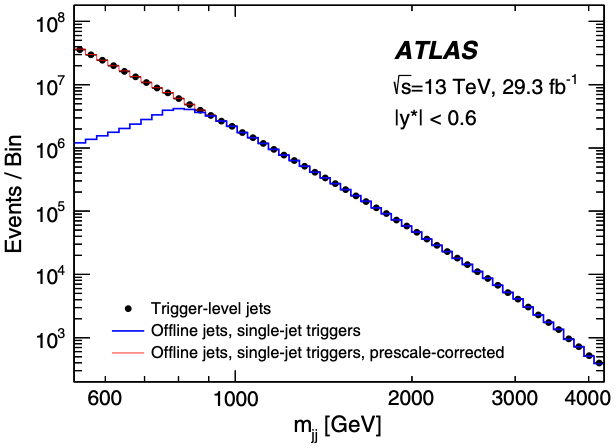
\includegraphics[width=0.55\linewidth]{images/atlas/ATLAS-TLA.png}
    \caption{Comparison of offline and trigger-level jet objects in ATLAS dijet spectra from Ref.~\cite{ATLAS:2018qto}. Trigger-level jets provide low $m_{jj}$ coverage without a requirement for a prescale correction.}
    \label{fig:trigger-level-efficiencies}
\end{figure}

%\subsubsection{The LHCb Turbo model}
Another example of such an approach is the LHCb Turbo model, a reduced-persistency event model, in which only the objects relevant to an HLT2 trigger decision (and any primary vertices) are persisted and saved to a dedicated stream~\cite{Aaij:2016rxn}. For inclusive triggers, which select events across many signals, many objects are still required. To circumvent this, inclusive trigger events are saved to a FULL stream, which can later be reselected by dedicated exclusive lines to extract only the relevant event objects. Many trigger-level objects may be required which are beyond the standard objects of a given decay, for example for flavour tagging. In such cases, selective persistency is applied, whereby an event is saved in the Turbo model with specified additional information, e.g., other tracks arising from a primary vertex, objects contained in a cone around the candidate, etc., A calibration stream (TurCaL) is a special use case of the selective persistence model, wherein only events dedicated to detector alignment and calibration are persisted~\cite{Aaij:2019uij}. % Discuss alignment further <- <- <-


%% COMPRESSION
% Baler? GPUs in ALICE, ML in CMS. Retina?

%model follows that for the fixed bandwidth, 10 GB/s due to offline storage resource constrains, the event rate can be increased, and therefore the physics sensitivity of the experiment, by reducing the event size saving only the ``interesting” part of the event. 

\section{Real-time analysis in physics results}
\label{sec:RTA_physics}
%Caterina having a first go, but students will edit further during circulation period

In this section, we briefly outline some of the physics analyses that have been performed by ATLAS, CMS and LHCb using real-time analysis (RTA) in Run~1 and Run~2. The success of such analyses has further motivated the development and adoption of RTA techniques in Run~3 trigger systems. %, as summarised in Table~\ref{trigger-table}.

% commenting out this table since it is a repetition of previous sections and it is unclear how it belongs to the physics section
\iffalse

\begin{table}[h!]
    \centering
    \begin{tabular}{c|p{0.75\linewidth}}
        \thickhline
        \small{\textbf{Experiment}} & \textbf{Summary} \\
        \hline\hline
        \multirow{3}{*}{\small{ALICE}}
            & \small{The ALICE trigger system provides timing to synchronise data from continuous and discrete subdetector readout systems. A software trigger then performs the reconstruction of events, reduction of data volume and calibration of subdetectors (e.g., TPC). The upgrade of many subdetectors to read out data continuously provides a significant increase in the number of collisions which can be collected (i.e., those previously occurring during subdetector dead time).} \\
        \hline
        \multirow{3}{*}{\small{ATLAS}}
            & \small{ATLAS uses a hardware-based L1 trigger to reduce the overall event rate from $40$ MHz to $100$ kHz, using granular information from the calorimeters and the muon spectrometer. A software-based computing farm, the HLT, reduces the L1 output rate down to $\sim$ 1.2 kHz. The HLT makes an early rejection based on Regions of Interest information coming from the L1 decision. The second step utilises full detector reconstruction together with more detailed algorithms for the final selection.} \\ \hline
        \multirow{3}{*}{\small{CMS}}
            & CMS employs a two-level trigger system similar to that of ATLAS. L1 decisions are made on granular information from the calorimeters and muon system. However, the CMS HLT reads out the full detector instead of Regions of Interest. The CMS HLT software farm also comprises of GPUs. CMS also has a trigger dedicated to long-lived particles. \\ \hline
        \multirow{3}{*}{\small{LHCb}}
            & \small{The removal of the L0 trigger requires that HLT1 reduce the event rate by a factor of 30, achieved by the use of GPUs en masse. HLT2 performs offline-quality reconstruction and real-time calibration, with events then saved in the reduced-persistency Turbo format on which analysis can then be performed. Many analyses should receive an improved statistical sensitivity through higher trigger yields and systematic sensitivity by avoiding L0-related systematic effects.} \\
        \thickhline
    \end{tabular}
    \caption{Summary of LHC trigger systems providing input to the real-time analysis data streams.}
    \label{trigger-table}
\end{table}

\fi

% Further comment on Run 3?

%\textbf{Note: this section has not yet been reviewed by CMS SMARTHEP participants, please point out any inaccuracies during the comments period.}
%\subsection{CMS}

The data scouting stream in CMS has been in place since the LHC Run~1, and its first use in searches for dijet resonances is described in Ref. \cite{CMS-PAS-EXO-11-094}. RTA allows the reach of this search to be extended to resonances with masses as low as \SI{500}{\giga\electronvolt}
%as demonstrated in Figure~\ref{fig:trigger-level-efficiencies}, 
improving on the standard data-taking analysis that would only be sensitive to resonances with masses of 1 TeV and above\footnote{Other techniques also exist beyond RTA to reach lower resonance masses, e.g., by triggering on initial state radiation or considering boosted jets that contain the resonance products.}. The same search has also been performed with the 8 and 13 TeV centre-of-mass LHC datasets in Run~1 and Run~2, and described in Refs. \cite{CMS:2016ltu, CMS:2016gsl}, extending the reach to 500 GeV resonances. ATLAS also searched for dijet resonances using the Trigger Level Analysis (TLA) technique, with sensitivity for resonances with masses as low as 450 GeV, as described in Ref. \cite{ATLAS:2018qto}.

%CD: missing dijet+ISR? 

Searches for multijet resonances (new particles decaying in paired dijet and three jets each) also employ, for example in Ref. \cite{CMS-PAS-EXO-21-004}. RTA extends the reach of previous searches to the low mass region from 200 GeV down to 70 GeV for RPV squarks and gluinos. 

Long-lived particles (LLPs) predicted by beyond-SM models decay far from the point of collision, a signature distinct from the promptly decaying particles of the majority of LHC searches. LLPs are often rejected by standard reconstruction algorithms due to their unusual characteristics (e.g., display decay vertices)~\cite{llps}. As such, LLPs require dedicated selection techniques and searches, for example, in CMS real-time searches for dark photons and LLPs decaying into muons using Run~2 data.  Ref. \cite{CMS:2019buh} describes a search for dark photons decaying into dimuons that uses RTA in the 11.5-45 GeV mass range. In Ref. \cite{CMS:2021sch}, RTA enables access to the new phase space of low dimuon masses and non-zero displacement that would otherwise not be covered by standard searches.

%\subsection{ATLAS}

%\subsection{LHCb}

In LHCb, real-time analysis was motivated~\cite{Gligorov:2018fuk} by the size of the LHC production cross-section of hadrons containing a charm 
quark. Because this cross-section is so large, it is not possible to record all signal decays of charmed hadrons to permanent storage while keeping the full detector information for each event. Therefore, these decays must be fully reconstructed and selected in real-time, requiring accurate and up-to-date detector alignment and calibration in the real-time processing to keep systematic uncertainties under control. This is particularly crucial since LHCb has a unique ability to probe CP violation in charm hadrons to the $10^{-5}$ level or better, requiring a corresponding control of systematics. For this reason, LHCb implemented the full offline-quality reconstruction, alignment, and calibration~\cite{Dujany:2015lxd, Aaij:2016rxn, Borghi:2017hfp, LHCb:2018zdd, Aaij:2019uij} of the detector within its real-time processing (specifically the software trigger) during Run~2, and adopted real-time analysis as the baseline model~\cite{LHCbCollaboration:2319756} for the majority of the collaboration's physics programme from Run~3 onwards. In Run~2, almost all analyses of charm hadrons, as well as certain searches for BSM states (most notably dark photons), were carried out using real-time analysis.
\section{Outlook on HL-LHC Upgrade}


% ATLAS+CMS to 1 level
% LHCb timing info?
% ALICE ???
% Possible approaches
% TDRs?

Following the conclusion of Run~3 (expected 2025), the LHC will enter the HL-LHC operational phase (expected 2029), with the installation of many detector upgrades in the interval. Accelerator upgrades will increase the LHC instantaneous luminosity up to \SI{7.5e34}{\per\square\cm\per\second}, a factor ten increase on the design luminosity. Access to this increased luminosity will allow the experiments to collect datasets an order of magnitude larger. This enormous increase in sample size enables the experiments to push both the precision and intensity frontiers of research.

The HL-LHC operation poses a series of challenges to the continued efficient operation of the trigger systems of the LHC experiments. For example, in ATLAS and CMS, pile-up is likely to increase to between 140 and 200 proton-proton interactions~\cite{ATLAS:pileup} from an average value of 55 in Run~3. As the occupancy and complexity of each event increases, so will the processing time required to make effective trigger decisions. %Increasing L1 and HLT trigger rates? here
The increase in event complexity brings an associated expansion in the memory footprint/bandwidth requirements. 
Furthermore, since QCD cross-sections scale linearly with pile-up, bandwidth limitations will result in significantly reduced fractions of low-energy jet selection, in turn hindering the sensitivity of low-energy jet searches~\cite{albrecht2018hep}.

In ATLAS and CMS, several improvements and innovations in both detector/hardware and software are under development targeting HL-LHC~\cite{hl-lhc}.

The upgrades to the sub-detectors will improve trigger performance (e.g., MIP/HGCAL in CMS~\cite{cms2019mip, cms2017phase-hgcal}, Calo~\cite{ATLAS:ECAL, ATLAS:HCAL}/Muon~\cite{ATLAS:Muon} in ATLAS L1, HGTD~\cite{ATLAS:HGTD}/ITK~\cite{ATLAS:ITKPixel, ATLAS:ITKStrip} in ATLAS HLT), or permit previously inaccessible combinations of sub-detectors (e.g., New Tracker in CMS~\cite{collaboration2017phasecms}). Additionally, upgrades to onboard electronics (e.g., FELIX in ATLAS~\cite{ATLAS:FELIX, ATLAS:TDAQ}) will handle the increased readout requirements as well as the increased complexity of events by allowing an increased L1 latency. Such increases in readout capacity will also be of vital importance as new/upgraded subdetectors will further increase readout requirements (e.g., HGCAL in CMS~\cite{cms2017phase-hgcal}).
In both experiments, there is an intense focus on heterogeneous computing architectures and their application in the real-time processing of data~\cite{ATLAS:c-and-s-roadmap,bocci2020heterogeneouscms}. ASICs and FPGAs, traditionally used in the initial stages of the data pipeline, are being deployed more widely and in diverse use cases. Migration of parallelisable tasks to GPUs is projected to reduce the power consumption, computational cost and wall time of the present trigger menus~\cite{cms-GPU-clustering}. 

Current software trigger algorithms have also been subject to scrutiny and the developments here are in many cases quicker to iterate than hardware upgrades. All of the algorithmic improvements would be too numerous to list here. We include just the following examples for brevity.
The ATLAS experiment intends to use novel GNN models to reduce resource consumption in track reconstruction~\cite{Caillou:2815578}, to be deployed on dedicated GPU cores in the new HLT.
In the CMS experiment the PF algorithm, described in Section~\ref{sec:Algorithms_PFlow}, will be launched inside the new L1 trigger in Run~4, and a correlator trigger will make use of tracks that are read out at \SI{40}{MHz} for the first time. A pile-up mitigation algorithm (PUPPI) will be used in L1 - requiring primary vertex identification.

In the HL-LHC paradigm, the use of specialised data streams based on reduced event content—Data Scouting in CMS~\cite{ardino202340cms,tomei2020cms,badaro202040cms}, TLA in ATLAS~\cite{ATLAS:TLA}, Turbo in LHCb~\cite{Aaij:2019uij}—will be expanded.
% NOT HAPPY WITH PREV PARA


%CMS
%https://cds.cern.ch/record/2714892
%https://arxiv.org/pdf/2010.13557.pdf %CMS track in trigger
%atlas
%https://cds.cern.ch/record/2285584

The LHCb and ALICE experiments will not make fundamental changes to their current running strategy for Run~4. Rather, major upgrades are scheduled for LS4 in preparation for Run~5 (to commence in 2035)~\cite{CERN-LHCC-2021-012, alice_loi_hl_lhc}.

\section{Conclusion}

The trigger systems at the major LHC experiments have undergone a continuous evolution throughout their operation in Run~1 and Run~2. Significant upgrades have been implemented and proposed to address the challenges posed by the current Run~3 and future high luminosity conditions. The triggers now take advantage of modern hardware developments in the sub-detector readouts and novel data processing software including contemporary machine learning developments. The result today is a more robust, flexible and efficient trigger system, better able to accommodate future requirements.

In Run~3, the major LHC experiments leverage their experience from Run~1 and Run~2 to tackle increased data challenges. In particular, upgrades to these experiments and their respective trigger systems take advantage of recent advances in hardware technologies, with software frameworks redesigned to better capitalise on such upgrades. New and optimised software frameworks also provide implementations for faster and more capable algorithms for reconstruction, selection and data manipulation. Overall, this experience will be integrated into the plans for Run-4, also taking advantage of new detectors and new trigger hardware capabilities. 



\clearpage
\section*{Acknowledgements}
%This is important, as it acknowledges our funding. 
This work is part of the SMARTHEP network and it is funded by the European Union’s Horizon 2020 research and innovation programme, call H2020-MSCA-ITN-2020, under Grant Agreement n. 956086. 

\bibliography{references, references_intro, references_LHCb, references_ALICE, reference_ATLAS, references_CMS, references_RTA, references_HLLHC}
\bibliographystyle{JHEP}

%\section*{Appendix}

\subsection{ATLAS detector}

The ATLAS detector\cite{ATLASMachine} is a general-purpose detector consisting of several sub detectors covering nearly all the area around the collision point. The detectors consist of the inner detector(ID), electromagnetic and hadronic calorimeters and a muon system. A small superconducting solenoid surrounds the inner detector with three large superconducting toroids(one around the barrel and two in the endcaps) around the calorimetry.

The inner detector surrounds the beam pipe, has a 2T axial magnetic field and measures momentum in the $|\eta| < 2.5$ region. The detector consists of three sub-detectors pixel, silicon microstrip and transition radiation trackers. The pixel tracker is situated closest to the beam pipe and is designed for a high-radiation environment. The highly granular detector makes on average 4 measurements per track. Following the pixel is the silicon microstrip detector which one average makes 4 measurements resulting in 4 space points. %Why?
The transition radiation tracker(TRT) surrounds the semiconductor detector in the barrel region(only barrel???) and consists of 4 mm drift straw tubes, generating trackick up to $|\eta| < 2.0 $. A track typically registers 36 hits per track in the TRT.

The calorimetry of ATLAS surrounds the solenoid and the ID with a coverage of $|\eta| < 4.9$. The electromagnetic calorimeter covers the barrel region($|\eta| < 1.475$) and the endcaps($1.375 < |\eta| < 3.2 $) with high-granularity lead/liquid-Argon(lAr) calorimetery. The hadronic section consists of tile calorimetry in the barrel and extended barrel regions($|\eta| < 1.7 $), the tile calorimetry use scintillating tiles as the active material and steel as the absorber. Additionally, the covered region is extended using an end-cap calorimeter covering $1.5 < |\eta| < 3.2 $ with lAr as the active material and copper absorbers. Finally, a dense forward calorimeter coveres the forward region inside the hadronic end-cap up to $|\eta| < 4.9 $.

The muon spectrometer covers the outermost parts of the ATLAS detector, the deflection of the muon tracks by the magnet system is use for the $p_T$ meaurements. The muon spectrometer consist of four sub-systems in three layers(cylindrical around beam axis in the barrel and perpendicular to the beam axis in the end-cap): Monitored Drift Tubes(MDT) and Cathode Strip Chambers(CSC) for precision tracking and Resistive Plate Chambers(RPC) and Thin Gap Chambers(TGC) for triggering.





\end{document}


\section{Introduction}
%\color{blue}Danielle
%\color{black}




\subsection{Hardware and software usage in the LHC triggers}
\color{red} \textbf{These sections may be summarized and merged into the appropriate experiment sections.}
\color{black}
% intro (try to explain why there are different needs)
% see https://www.annualreviews.org/doi/10.1146/annurev-nucl-102115-044713

\subsubsection{ATLAS and CMS}
The ATLAS and the CMS experiments have a similar trigger system with a two-level structure, consisting of a Level-1 (L1) hardware-based trigger and a software based high-level trigger (HLT).
The general hardware-software architecture did not change from Run 1 to Run 3.
For both experiments, there were upgrades between the three LHC runs to adapt the TDAQ systems to face the increased data rates and beam energies reached by the LHC.

% ATLAS
In the trigger system of the ATLAS experiment event data are initially read out via dedicated electronics, that perform initial pulse shaping, analogue-to-digital conversion and aggregation of the signals received from on-detector sensors.
The part of these data coming from the calorimeter and the muon systems is used by the L1 trigger, built in custom electronics, to perform a fast selection searching for signatures such as large electromagnetic energy deposits or high-$p_\mathrm{T}$ muon tracks.
At this stage in Run 1 the overall event rate was reduced from \SI{20}{\mega\hertz} to a maximum of \SI{75}{\kilo\hertz} and the L1 decision had to reach the front-end electronics within a latency of \SI{2.5}{\micro\second} after the associated bunch-crossing \cite{PanduroVazquez:1954156}. In Run 2 and Run 3, the acceptance rate of the L1 trigger goes up to \SI{100}{\kilo\hertz}, which is the maximum detector read-out rate, starting from a bunch crossing rate of about \SI{40}{\mega\hertz}. The L1 trigger was upgraded for Run 3. During the upgrade, trigger latency was a critical parameter, as the majority of the detector front-end electronics will not be replaced before LS3. The trigger latency is now \SI{2.2}{\micro\second}.
For each L1-accepted event, the front-end electronics read out the event data for all detectors. These data are sent first to ReadOut Drivers (RODs), to perform the initial processing and formatting, and after to the ReadOut System (ROS) to buffer the data, and finally to the HLT. The ROS is the first part of the DAQ chain to make partial use of non-custom hardware.
To avoid the transferring of unwanted data, the event components used as part of the L1 decision are used to build regions-of-interest (RoIs) in the detector to be investigated by the HLT. These regions are based on geographical locations within the detector in which interesting signals are identified and assembled via dedicated hardware. 
In Run 1 the HLT was formed by three processing farms: the Level-2 (L2) trigger, the event builder (EB) and the event filter (EF). These systems were all implemented on commercially available server PCs using entirely software-based selection algorithms. The data were transferred between the farms via high speed Ethernet-based networks.
The L2 trigger processed the RoI information using software based selection algorithms, with a peak output event rate of \SI{6.5}{\kilo\hertz}. Then the data were sent to the EB farm, which requested the full readout of the selected event from the ROS and then passed the data to the final EF farm, where more complex selection algorithms were applied. Events passing this final stage were written to permanent storage. For Run 2, the L2-EF structure has been simplified and the two processing steps conceptually merged: before, L2 algorithms on a dedicated farm seeded processing in a separate EF farm, whereas now there is one common HLT farm with each node capable of performing all processing steps. The advantages are that it is no longer needed to transfer the data from one farm to another and that all the cores of the farm can process all HLT processes. This allows much more efficient resource distribution and load balancing and increases the maximum rate.
The peak data rate recorded to disk after the HLT in Run 1 was of order \SI{1}{\kilo\hertz}, increased to an average of \SI{1.2}{\kilo\hertz} in Run 2.\\
% still missing references:
% \cite{ATLASMachine}
%https://arxiv.org/abs/2007.12539, atlas run2 operations
% https://inspirehep.net/files/61e32e7984648e8fa66ffdf84e2ae6fe
% TDR for phase 1, 1.3 Present System and Planned Upgrades
% https://inspirehep.net/files/0e4a1261fb1a366a088efe45ccd0b7c5
\vspace{0.3 cm}

% CMS 
Similarly to the ATLAS, the first level (L1) of the CMS trigger is implemented in custom hardware, and selects events containing candidate objects, e.g., ionization deposits consistent with a muon, or energy clusters consistent with an electron, photon, $\rm \tau$ lepton, missing transverse energy, or jet. The L1 trigger takes input from the calorimeters and the muon system. 
Trigger primitives are generated on the front-ends of the subdetectors and then processed in several steps before a final decision is rendered in the global trigger.
The thresholds of the L1 trigger are adjusted during data taking based on the value of the LHC instantaneous luminosity, to restrict the output rate to the upper limit imposed by the CMS readout electronics of \SI{100}{\kilo\hertz}. The trigger latency is \SI{4}{\micro\second}.
The L1 trigger was majorly upgraded for Run 2: all electronic boards of the system have been replaced, allowing more sophisticated algorithms to be run online; the global trigger is now able to perform complex selections and to compute high-level quantities, like invariant masses.
For Run 3, a large effort was invested to develop new features and new trigger algorithms oriented to long-lived particle (LLP) signatures and rare signals at L1. Thanks to the upgrades of the hadronic calorimeter (HCAL), new inputs from the L1 calorimeter objects like the timing and the depth information can be exploited for physics purpose.
Events accepted at L1 are passed to the second level (high-level trigger, HLT).
The HLT is a streamlined version of the offline reconstruction software running on a computer farm and selects events for offline storage.
In Run 1, the farm was formed of commodity CPUs. The HLT hardware consisted of a processor farm using commodity PCs running Scientific Linux. 
The subunits were called builder and filter units. In the builder units, event fragments are assembled to complete events. Filter units then unpack the raw data and perform event reconstruction and trigger filtering. The average output rate was \SI{400}{\hertz}.
For Run 2, the algorithms that run in the HLT went through big improvements. In particular, new approaches for the online track reconstruction lead to a drastic reduction of the computing time, and to much improved performance. The output rate was increased to \SI{1}{\kilo\hertz}, with a latency of few hundred milliseconds.
For Run 3 the HLT underwent major improvements: a new tracking based on the optimized pixel track reconstruction, known as Patatrack, has been implemented. The tracking can now be offloaded to GPUs. The new HLT farm is composed of two-hundred nodes with $25600$ CPU cores and $400$ GPUs in total. Thanks to the increased usage of GPUs, the HLT algorithms can be redesigned for parallel architectures. For the start of Run 3, the calorimeter and pixel local reconstruction plus the pixel tracking have been ported to GPU and CMS is currently offloading \SI{30}{\percent} of the HLT reconstruction to GPU. The GPU reconstruction has been implemented and fully commissioned both offline and online.
% still missing references:
%https://arxiv.org/pdf/1609.02366.pdf run 1
%https://pos.sissa.it/314/523/pdf run 2
%http://cds.cern.ch/record/2842439/files/CR2022_256.pdf run 3

\subsubsection{LHCb}
% Run 1
%https://cds.cern.ch/record/1129809/files/jinst8_08_s08005.pdf
The detector geometry and scope of the physics program of the LHCb experiment, and thus the trigger system, are significantly different from the ATLAS and CMS ones.
During Run 1, LHCb operated at an average levelled luminosity of $2\times10^32 \,\rm cm^{-2} s^{-1}$, that is much lower than the maximum design luminosity of the LHC.
The effective collision rate and so the incoming data rate was about \SI{15}{\mega\hertz}. The rate of events written to storage was reduced by the trigger to about \SI{5}{\kilo\hertz}. % second ref
The LHCb trigger system was composed by two levels: the Level-0 (L0) hardware-based and the High Level Trigger (HLT), software-based. Similarly to the ATLAS and CMS L1 triggers, the LHCb L0 trigger was implemented using custom electronics, operating synchronously with the $40 \,\rm MHz$ bunch crossing frequency, while the HLT was executed asynchronously on a processor farm, using commercially available equipment. 
The trigger was optimised to achieve the highest efficiency for the events selected in the offline analysis, using event selections based on the masses of the rare $B$ mesons, their lifetimes and other stringent cuts to enhance the signal over background. The L0 trigger reduced the rate from \SI{40}{\mega\hertz} to \SI{1}{\mega\hertz}, with which the entire detector could be read out. A Level-0 Decision Unit (DU) collected all the information and derived the final L0 trigger decision for each bunch crossing. All L0 electronics were implemented in fully custom-designed FPGA boards which made use of parallelism and pipelining to do the necessary calculations with sufficient speed.
The HLT consisted of a C++ application which ran on every CPU of the Event Filter Farm (EFF), which contained up to $2000$ computing nodes. The HLT reduced the event rate from \SI{1}{\mega\hertz} to \SI{2}{\kilo\hertz}, making use of the full event data. It was subdivided in two stages: the HLT1 and the HLT2. The purpose of HLT1 is to reconstruct
particles corresponding to the Level-0 objects, with the general requirement of candidate tracks with a combination of high $p_\mathrm{T}$ and/or large impact parameter. HLT1 reduced the rate to about \SI{30}{kilo\hertz}, that is sufficiently low to allow for a full pattern recognition on the remaining events. At this rate, the HLT2 performed a combination of inclusive trigger algorithms (where the $B$ decay is reconstructed only partially), and exclusive trigger algorithms (which aim to fully reconstruct $B$-hadron final states). Selection cuts at HLT2 were relaxed compared to the offline analysis, in order to be able to study the sensitivity of the selections and to profit from refinements due to improved calibration constants. A large fraction of the output bandwidth is devoted to calibration and monitoring.

% about run 1 from second reference
% Almost all events accepted by the HLT were sent to permanent offline storage containing all raw information from the detector. The online event reconstruction, i.e. the one performed in the trigger, was simpler than the one used offline, i.e. the one performed on the LHC Computing Grid to recreate particles in the event from the raw data. This was done in order to fulfil the tight time constraints imposed in the trigger. This implied the usage of a preliminary version of the alignment and calibration and a faster, but less performing, track reconstruction and particle identification determination. The final detector calibration and alignment parameters were obtained offline on triggered data and applied afterwards during scheduled campaigns where the data were centrally re-processed. During these campaigns, all the events were re-reconstructed offline using a different version of the reconstruction software that allowed to achieve the best performance regardless of the timing required. Clearly, this strategy costs a lot of computing resources, since the reconstruction software was run twice and could also cause a loss of imperfectly reconstructed data in the trigger due to the usage of preliminary calibration and alignment.

% Run 2
%https://cds.cern.ch/record/2310660/files/epjconf_icnfp2017_01016.pdf
Due to the change of the bunch spacing to \SI{25}{\nano\second}, in Run 2 the effective collision rate doubled compared to Run 1. This required a more efficient trigger strategy, since the extension of the offline processing resources did not scale with the increased data rate.
To achieve this, the new trigger system was designed to allow to have the same offline-data quality already at the trigger level, which is a difficult challenge due to the time constraints imposed by the trigger. The major change to the trigger strategy that allowed to achieve this goal is that the processing of the HLT2 was completely deferred, in order to optimise the usage of the EFF. The EFF combined storage space (of about $10 \,\rm PB$ in 2016) could accommodate up to two weeks of LHCb data taking in nominal conditions. It was possible to use the time when the LHC was not in stable running, in which the farm is not busy, to process the HLT2 data. This strategy allowed to have more time to process a single event and gives the opportunity to calibrate and align the subdetectors in pseudo real-time using data from HLT1. This continuous calibration and alignment, which only updates the alignment constants when necessary, enables an offline-quality reconstruction at trigger level. This, combined with the doubling of the trigger farm capacity and the improved track reconstruction, allowed to have the same online reconstruction as the offline one and to increase the output rate to \SI{12.5}{\kilo\hertz}. 

% Run 3
% https://lhcb.github.io/starterkit-lessons/first-analysis-steps/dataflow-run3.html
% see links to Run 1 and Run 2
In Run 3, the instantaneous luminosity is increased by a factor of five. The L0 hardware trigger has a rate limit of \SI{1}{\mega\hertz}, which would be a limitation with this increase in luminosity.
Such a low rate could be only achieved by having tight hardware trigger thresholds, that is particularly inefficient for fully hadronic decay modes, and a major limitation for the physics output of LHCb.
Thus, LHCb underwent a major upgrade: during Run 3, the L0 trigger stage was completely removed, moving to a fully-software based trigger. This implied significant changes in the data processing chain of the experiment both online and offline.
The front-end and readout electronics of all sub-detectors had to be replaced, to be able to operate at the average non-empty bunch crossing rate in LHCb of \SI{30}{\mega\hertz}.
The software trigger is still implemented in two steps: the HLT1, which performs partial event reconstruction and simple trigger decisions based on kinematic and topological variables to reduce the data rate, and HLT2, which performs the more computationally expensive full reconstruction and completes trigger selection also exploiting particle identification information in the trigger selections. One of the most important tasks of building the events is track reconstruction, which is a parallelizable process: for this purpose, HLT1 in Run 3 is implemented as part of the Allen project and runs on GPUs. % ref to Allen

\subsubsection{ALICE}
The ALICE experiment has the prime objective of studying heavy ion interactions at LHC energies. The strong-interaction cross section in these conditions is very large, but the maximum luminosity available for ion collisions is lower than the one available for pp collisions ($10^{27} \,\rm cm^{-2}s^{-1}$ for PbPb versus $10^{34} \,\rm cm^{-2}s^{-1}$ in ATLAS and CMS for pp interactions). In addition, heavy ion interactions are characterised by very high event multiplicities. Since the physics aims and running conditions for the ALICE experiment are different from those of the other experiments at the LHC, also the trigger approach is different. 
In Run 1, the ALICE trigger system had three levels of hardware trigger: the Level-0 (L0, with a latency of \SI{1.2}{\micro\second}), that inputs the Level-1 stage (L1, with a latency of \SI{6.5}{\micro\second}), that inputs the Level-2 stage (L2, with a latency of \SI{100}{\micro\second}).
The Central Trigger Processor (CTP) consists of six different board types, all implemented in 6U VME, housed in a VME crate with a custom J2 backplane for transmission of trigger signals from one board to another. A seventh board type, the Local Trigger Unit (LTU), serves as the interface between the CTP and the detectors. There is one LTU per detector.
In Run 2 this system was upgraded with the addition of the LM level (latency: \SI{800}{\nano\second}), used to provide a minimum bias-like trigger to be used to activate the TRD electronics, which are kept switched off when not required to reduce heat dissipation.
The last step of the trigger system is, as for the other experiments, the software-based high-level trigger (HLT). The HLT consists of a PC farm of up to $1000$ multi-processor computers. The data processing is carried out by individual software components running in parallel on the nodes of the computing cluster.
In Run 3 the rate of PbPb collisions in ALICE increased from about \SI{8}{\kilo\hertz} to \SI{50}{\kilo\hertz}. Thus the trigger system had to undergo major upgrades.
The physics signals of interest to ALICE are in general complex to separate, and therefore not suitable to hardware triggers: this is why for Run 3, ALICE uses a continuous readout, applying a minimum bias trigger to the data stream to flag events and using sophisticated filters on fully reconstructed events. In order to do this, most but not all detectors upgraded to a continuous readout. Since not all the detectors are upgraded, the new system retains backwards compatibility.
The CTP has a completely new hardware, advances in the processing power of FPGAs since the time when the original CTP was designed.

% References
% Run 1
% K. Aamodt et al, The ALICE experiment at the CERN LHC, JINST 3 (2008) S08002
% Run 2
% B. Abelev et al., Upgrade of the Readout and Trigger System, CERN-LHCC-2013-019
% Run 3
% https://pos.sissa.it/313/149/pdf
\newpage
\subsection{Trigger system of the LHCb experiment}

The LHCb experiment is a heavy-flavour experiment operating in the forward region, searching for new physics through precision studies of the properties of heavy-flavour decays, in particular CP- and flavour-violation. Following the upgrade of the detector prior to Run~3, the LHCb detector operates as a general-purpose forward detector. The LHCb trigger system was redesigned for Run~3, removing the low-level Level 0 (L0) hardware-based trigger previously employed in Runs 1 and 2. The simplistic cut on $p_{T}$ implemented in the L0 trigger could not discriminate between signal and background for hadronic signals, which would have resulted in a effeciency loss as seen in Fig. \ref{fig:LHCbL0TriggerYield}. As such, the LHCb trigger consists solely of a HLT, split between two stages: HLT1 and HLT2~\cite{Aaij:2019uij}. Following the removal of the L0 trigger, LHCb event readout has increased from \SI{1}{\mega\hertz} to \SI{30}{\mega\hertz}. During Run~2, HLT1 and HLT2 were decoupled to allow HLT1 to run synchronous to data-taking and HLT2 to run asynchronously, enabling  detector calibrations between the steps to improve reconstruction performance to offline quality~\cite{LHCb:Albrecht_2015}. 

\begin{figure}[h!]
    \centering
    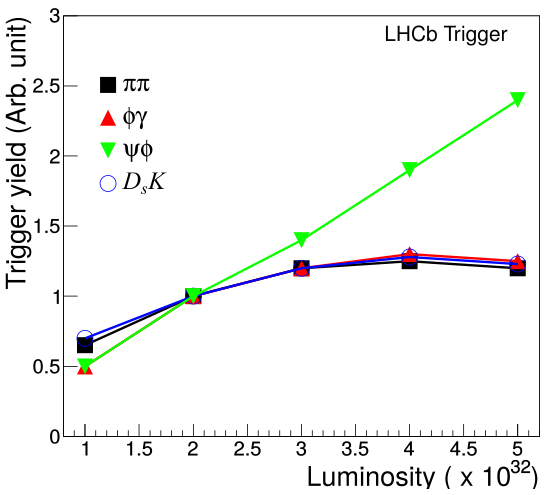
\includegraphics[width=0.55\linewidth]{images/lhcb/LHCb-L0-yield.png}
    \caption{Trigger yield per mode of interest with the Run 2 trigger configuration from Ref.~\cite{LHCb:upgrade-piucci}. Any increase in luminosity from accelerator upgrades is suppressed by the L0 trigger in all modes but $\psi\phi$ (i.e., non-muonic modes).}
    \label{fig:LHCbL0TriggerYield}
\end{figure}

HLT1 was upgraded throughout Run 2 to perform a partial reconstruction of the full detector readout. To achieve this, the reconstruction algorithm was upgraded to be able to run on GPUs hosted on the same event-building servers that host the FPGA cards required to receive data from the detector at 30 MHz~\cite{LHCb_Allen_GPU}. Reconstructed, selected events are propagated to a buffer at an event rate of ${\sim}\SI{1}{\mega\hertz}$. HLT2, implemented as a CPU farm known as the Event Filter Farm (EFF), takes as input the most recent detector alignment and calibration, reconstructing events in full offline quality for detailed selection. This selection reduces the event rate to \SI{100}{\kilo\hertz}, corresponding to an output bandwidth of \SI{10}{\giga\byte\per\second}~\cite{lhcb_hlt2_storage_run3}.

\subsection{Trigger system of the ALICE experiment}
The ALICE experiment is dedicated to the study of heavy-ion collisions at the LHC, with a focus on studies of quantum chromodynamics in energy-dense environments (e.g.,  quark-gluon plasma)~\cite{alice-performance-paper-run1}. To study such environments, ALICE studies p-p, p-Pb and Pb-Pb collisions at frequencies of \SI{1}{\mega\hertz}, \SI{500}{\kilo\hertz} and \SI{50}{\kilo\hertz}, respectively \cite{alice-trigger-run3}. Heavy ion collisions result in a very high multiplicity of particles, with ${\sim}\SI{700}{\mega\byte}$ of raw data per collision event collected by the ALICE experiment \cite{alice-rta-trigger}. The ALICE detector is barrel-shaped, containing concentric particle tracking and identification systems, and a forward muon spectrometer. At the core of the barrel is a Time Projection Chamber (TPC) vital to tracking performance, contributing the majority of the event size (\SI{95.3}{\percent} and \SI{91.1}{\percent} of total data volume in Pb-Pb and p-p collisions, respectively).

The ALICE trigger was upgraded ahead of Run~3 to facilitate continuous readout of subdetectors at collision frequency. The Central Trigger System (CTS), is responsible for the synchronisation of raw detector readout. The CTS transmits aggregated data and trigger signals to the HLT. The HLT then performs event reconstruction, data volume reduction and subdetector calibration, processing data at a maximum rate of \SI{48}{\giga\byte\per\second} to achieve an output throughput of up to \SI{12}{\giga\byte\per\second}~\cite{alice-rta-trigger}.

\section{\label{sec:ATLAS}Trigger system of the ATLAS experiment}
\subsection{ATLAS Trigger and data acquisition}

The ATLAS trigger and data acquisition(TDAQ)\cite{ATLAS-TDR-PhaseI} system is designed to process and filter a large amount of data coming from the LHC collisions. At 40 MHz of bunch crossings, approximately 40 TB/s of data is produced that needs to be heavily reduced to $\approx$1 kHz/1 GB/s. The vast majority of the collisions in the ATLAS detector is of minimal interest to the ATLAS physics program, the job of the TDAQ is therefore to process and save only the data needed for analysis. 

\subsubsection{HLT}

The HLT is a software-based computing farm which processes the 100 kHz coming from the L1 trigger down to on average 1.2 kHz rate and 1.2 GB/s of throughput. The trigger first makes an early rejection based on fast trigger algorithms which are seeded by the RoI information coming from the L1 decision. The second step is then followed by a more detailed part where the algorithms are close to offline reconstruction level. The HLT computing farm consists of approximately 40000 Processing Units(PUs) that make decisions within a few hundred milliseconds\cite{ATLASTriggerRun2}.

\subsection{Run 3}

For Run 3 the LHC has upgraded its luminosity to $\mathcal{L}$= $2.0\times10^{34} \; \text{cm}^{-2}\text{s}^{-1}$ for ATLAS, this increase in pile-up gives substantial challenges for the detectors systems and the trigger system. Detector upgrades in the muon system will help to reduce fake muons in the high $\eta$ region for the L1 trigger. The L1Calo has been completely replaced with new FPGA-based triggers which utilizes the increased trigger-level granularity of the ECAL readout. Upgrades have also been made to the detector read-out system with the new FELIX card and to the HLT with multithreading improvements.

\subsubsection{L1Muon}

The L1Muon trigger has been improved with hardware upgrades in the New Small Wheel(NSW) and the RPC BIS78 both located just outside the calorimetry in the endcap. The aim of these upgrades is to add an additional coincidence measurement in the $2.7>\eta> 1.0 $ region to reduce the fake muon rate. These fake muons spiral into the endcap from further down the beam pipe from the primary vertex and create a fake straight track in the end-cap TGC detectors. The expected reduction of the fake muon rate have been simulated for the L1\_MU20 trigger line. A $\approx 45 \%$ reduction in the rate below $p_{\text{T}}$ 20 GeV is expected from Run 2 to Run 3, with a negligible efficiency loss\cite{Ventura:2841379}.
%Maybe remove 45% part, a bit too specific?
\subsubsection{L1Calo}

The L1Calo trigger underwent a complete replacement leading into the increased luminosity environment of Run 3. The basis of the L1Calo upgrade is the newly installed output electronics in the lAr electromagnetic calorimeter increases the granularity available at trigger level. From trigger towers of ($\Delta\eta\times\Delta\phi=0.1\times0.1$) during Run 2 to 10x the granularity with a mix of new($\Delta\eta\times\Delta\phi=0.025\times0.1$) and old granularities with different segmentation along the r-axis. This increase in granularity enabled the L1Calo hardware upgrade with a new system of FPGA-based Feature EXtractor(FEX) modules. The FEX modules exploits the increase in granularity with more complex algorithms to identify physics object in the challenging high luminosity environment. These new modules are split into three categories: electron(eFEX), jet(jFEX) and global(gFEX) feature extractors. The eFEX use the full calorimeter information to search for smaller electron, photon or tau-like signatures using the improved granularity to enhance the rejection of jet background. The detector data is distributed to the 24 ATCA-based modules. The upgrade gives a sharper turn-on curve for trigger line efficiencies and a potential lowering of the $E_{\text{T}}$ threshold due to lower rates. Unlike the eFEX, the jFEX does not demand the entire granular dataset. It comprises of 6 modules, designed for jet-like signatures and missing energy measurements. Compared to the previous Jet Energy Processor the jFEX has more flexibility, especially enabling regional correction for pileup effects. Finally, the gFEX processes the full detector data at a coarser granularity with a single module enabling jet-identification and missing energy measurement with larger jet object and full event correlations\cite{Mkrtchyan:2843493}.


\subsubsection{AthenaMT}

The Athena\cite{Athena:865624} software framework is used throughout the entire event data process, from trigger through simulation and reconstruction to physics analysis. The framework is based of the Gaudi\cite{Gaudi:200145} framework which is a inter-experiment and both ATLAS and LHCb uses it as base for there respective software frameworks. These frameworks were originally designed in the early 2000s which meant that the architectural design implemented a single-process and single-thread operational mode. Current day performance increase requires memory sharing and simultaneous processing. The multi-threaded Athena framework, AthenaMT\cite{Bielski_2020}, have been developed leading into Run 3 and enables both inter-event and intra-event parallelization and is based on Gaudi Hive using a scheduler based on Intel Thread Building Blocks(TBB). The sharing of event-independent data between threads provides improved memory handling and thereby increase in performance.
%This was a reasonable choice during the days where clock frequency followed Moore's law and memory price was decreasing logarithmically. 

\subsubsection{FELIX}

The Front-End LInk eXchange(FELIX) system is a data routing interface between detector readout electronics and the trigger to the data acquisition system. FELIX uses PC-hosted FPGAs on PCIe boards to go from custom serial links to commodity switch network using commercial technologies(Ethernet or Infiniband). After L1 decision the data is then sent to the SWROD(SoftWare ReadOut Drivers) which is in charge of data processing, aggregation and monitoring after it then sends it to the HLT. The improvement of the FELIX system is the use of commodity computing over custom designs reducing the complexity of the system and the effort needed in maintaining and upgrading it. The FELIX system will be installed for the NSW, lAr calorimeter, L1Calo and RPCBIS78 detector systems.
%Add reference!!

\subsection{HL-LHC}

The HL-LHC is expected to begin in 2026, with a nominal peak instantaneous luminosity of $\mathcal{L}= 5 \cdot 10^{34} \; \text{cm}^{-2}\text{s}^{-1}$, which will give an average of 140 inelastic proton-proton collisions per bunch crossing. This extensive increase in the number of collisions per event will pose a large challenge for the ATLAS TDAQ system. The design of the upgraded system shown in figure \ref{fig:TriggerHL-LHC} takes advantage of increased precision from detector upgrades in calorimeters, muon detectors and the new Inner Tracker. The Phase-II upgrade will partly continue on the Phase-I upgrade especially in readout, calorimetry and muon trigger systems. The FELIX system initially installed for certain components during Run 3 will now be expanded to all detector systems to handle the increased throughput.

\begin{figure}[t!]
    \centering
    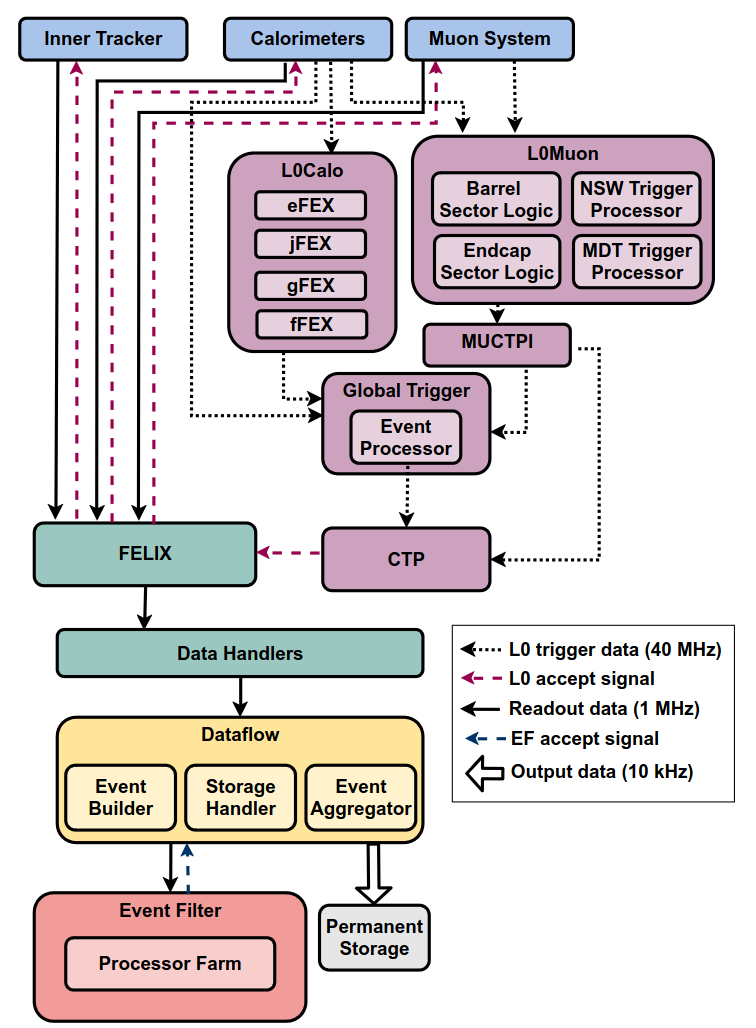
\includegraphics[width=0.7\linewidth]{images/atlas/ATLASHL-LHCTriggerSchematic.png}
    \caption{The trigger schematic for HL-LHC trigger architecture\cite{ATLAS:TDAQ-TDR-EF}.}
    \label{fig:TriggerHL-LHC}
\end{figure}

\subsubsection{Detector upgrades}

The Inner Tracker(ITk)\cite{CERN-LHCC-2017-021,CERN-LHCC-2017-005} will replace the current Inner Detector in the same volume with an increased acceptance from $|\eta|<2.5$ to $|\eta|<4$, better $p_\text{T}$ resolution and similar tracking efficiency but at the more challenging pile-up of 200 during HL-LHC. It accomplishes this through a fully silicon detector with 13 $\text{m}^2$ of pixel detector(inner system, outer barrel and outer end cap) and 168 $\text{m}^2$ of strip detectors(barrel and end cap) which ads up to 5.1 billion channels. The layout generates at least 9 silicon hits per track within acceptance and radiation tolerance up to 1e16 neq$/\text{cm}^2$ for the inner pixel layer.

The High Granularity Timing Detector(HGTD)\cite{CERN-LHCC-2020-007} aims to improve pile-up rejection in the forward region ($2.4<|\eta|<4.0$) with two wheels located in front of the lAr end-caps at a $|z|= 3.5$ m. Timing resolution of 30-50 ps/track(up to 4000 $\text{fb}^{-1}$) enables the rejection of pile-up, this is enabled by radiation hard carbon infused Low Gain Avalanche Detectors(LGAD) sensors.


Both the lAr\cite{CERN-LHCC-2017-018} and Tile\cite{CERN-LHCC-2017-019} Calorimeters need new readout electronics due to the increase in radiation tolerance limits together with the increase in rates and latencies at the HL-LHC luminosity.

The Muon Spectrometer\cite{CERN-LHCC-2017-017} will need new trigger electronics for the first level of the trigger in both the RPCs and TGCs. All front-end electronics will be upgraded to enable readout/triggering at 40 MHz, these new electronics will also add hit information from the MDT into the L0 trigger to improve the turn-on efficiency. Additionally new MDT and RPC layers in the barrel region will improve trigger performance.

\subsubsection{TDAQ}

The L0 trigger system will benefit from the extensive detector upgrades but with a decision making architecture similar to the Run 3 system but at a readout rate of 1 MHz and a maximum latency of 10 $\mu$s. The L0Calo(Previously L1Calo) will consist of eFEX, jFEX and gFEX from Run 3 with upgraded firmware and potential modifications. A new forward FEX(fFEX) will be installed to reconstruct electrons and jets in the forward region, up to the coverage of the ITk. The L0Muon(Prevoiusly L1Muon) constist of Barrel(RPC) and Endcap(TGC) sector logic processors, NSW trigger processor and the MDT trigger processor. The muon sector feeds into the MUCTPI which then feeds into the global trigger together with L0Calo information. The global trigger refines the L0Calo and L0Muon information, executes topological algorithms that combine different signatures together similar to L1Topo and processes event-wide quantities. Finally, the CTP makes the L0 decision with the information it receives from the Global Trigger. The decision triggers the FELIX system which handles the readout into the second part of the trigger: The Event Filter(EF)\cite{CERN-LHCC-2017-020}. 

The EF(previously HLT) originally was planned as a CPU-processing farm together with a Hardware-based Tracking for the Trigger(HTT) co-processor. The HTT scenario was eventually removed\cite{ATLAS:TDAQ-TDR-EF} for a scenario with tracking in the CPU-farm with the potential for using hardware accelerators to optimize the farm. Accelerator performance studies are being done for several different tasks with the EF, mainly focusing on tracking but also includes GPU-based topological cell clustering for the calorimeter. The software framework upgrade consists of evolution of the framework but also more efficient algorithms. Most of this work can continue upon the AthenaMT framework upgrade done before Run 3 together with additional optimization of selection algorithms\cite{CERN-LHCC-2017-020}.

\section{\label{sec:CMS}Trigger System at the CMS Experiment}
The Compact Muon Solenoid (CMS) detector operates at the LHC\cite{collaboration2008cms}. Along with the ATLAS experiment it is one of the two general-purpose detectors in operation at the LHC used to study proton-proton (and lead-lead) collisions with a centre-of-mass energy of $13.6$TeV and at an instantaneous luminosity of up to $2 \cdot 10^{34} cm^{-2}s^{-1}$ in Run 3.
\par

At the Run 3 design luminosity a mean of around 50 inelastic collisions will occur in each bunch crossing with a frequency of around $40$MHz. Since the response and readout times of some detector elements may exceed the $25$ns spacing between bunch crossings the design and performance of the trigger is crucial to the physics data-taking operation.[citation?]


\subsection{The CMS Detector}

% At the centre of the CMS detector is a $13$m long, $3.8$T superconducting solenoid with a diameter of $6$m, that gives the experiment its name\cite{bayatian2006cms}. Inside the coil of the magnet the cylindrical structure of the detector is as follows: silicon pixel and strip trackers, a lead-tungstate scintillating-crystals electromagnetic calorimeter and a brass-scintillator sampling hadron calorimeter. The outermost layers of the detector, outside the solenoid, contain the muon system/detectors. There are 4 muon stations each consisting of several layers of aluminium drift tubes in the barrel and cathode strip chambers in the endcap region. In the forward regions of the detector the barrel calorimeter are complimented by further iron/quartz-fibre calorimeters increasing the pseudorapidity coverage.
% A more detailed description of the CMS detector, together with naming conventions, coordinate system definition and relevant kinematic variables can be found in \cite{cms_detector}. 


The central feature of the CMS apparatus is a superconducting solenoid of 6\unit{m} internal diameter, providing a magnetic field of 3.8\unit{T}. Within the solenoid volume are a silicon pixel and strip tracker, a lead tungstate crystal electromagnetic calorimeter (ECAL), and a brass and scintillator hadron calorimeter (HCAL), each composed of a barrel and two endcap sections. Forward calorimeters extend the pseudorapidity coverage provided by the barrel and endcap detectors. Muons are measured in gas-ionization detectors embedded in the steel flux-return yoke outside the solenoid. A more detailed description of the CMS detector, together with a definition of the coordinate system used and the relevant kinematic variables, can be found in Ref.~\cite{collaboration2008cms}. 
%Duplicated later?
% Events of interest are selected using a two-tiered trigger system. The first level (L1), composed of custom hardware processors, uses information from the calorimeters and muon detectors to select events at a rate of around 100 \unit{kHz} within a fixed latency of 4 \unit{\mu s} ~\cite{CMS:2020cmk}. The second level, known as the high-level trigger (HLT), consists of a farm of processors running a version of the full event reconstruction software optimized for fast processing, and reduces the event rate to around 1 \unit{kHz} before data storage~\cite{CMS:2016ngn}.




\subsection{The CMS Trigger}
As previously discussed the event rate at the LHC far exceeds the processing and storage capabilities of the four major experiments. 
Only a small fraction of the bunch crossings contain interactions of interest to the physics program of CMS. It is therefore the job of the CMS trigger system to separate the events to be saved amid the huge background event rate.
\par

The trigger system employed by the CMS collaboration reduces the event rate in two sequential steps of decision-making, the Level 1 and High Level Trigger.  


\subsubsection{L1 Trigger}
The first step in the trigger called Level 1 (L1) is characterized by its use of custom/bespoke hardware to drastically and rapidly reduce the event rate. Much of the L1 trigger logic is implemented in custom Application Specific Integrated Circuits (ASICs), Field Programmable Gate Arrays (FPGAs), Programmable Logic Devices (PLDs) and discrete logic such as memory Look-Up Tables (LUTs)\cite{cms2016cms,cms2020performance}.
\par

The initial L1 trigger decision occurs with a latency of $4 \mu$s and reduces the  rate from $40$MHz to a maximum of $100$kHz, limited by the detector readout. 
Crucially, the L1 hardware only has access to a coarse segmentation of data read-out from the calorimeters and the muon system as well as some correlation of information between these systems\cite{fontanesi2022cms}.


%maybe too long?
% As stated, the L1 trigger decision is made using simplified readout from the calorimeters (ECAL,HCAL,HF) and muon chambers (CSC, DT, RPC) that are called trigger primitives. All tracker information is not available to the L1 trigger. Trigger primitives are subsequently combined to form calorimetric towers and to link compatible muon hits together. These composite trigger primitives are then used to form the L1 trigger objects and the event achieves an L1 accept if the L1 trigger objects fulfill at least one of the pre-defined conditions of the L1 menu, as evaluated in the global trigger. The global trigger is the final part of the L1 trigger system and implements a menu of triggers/selection requirements on final L1 objects.
% See [ref] for a more detailed description of the working scheme of the TPs in L1.



\subsubsection{High Level Trigger}

The second step of the CMS trigger is the High Level Trigger (HLT). Implemented entirely in software running on a farm of commercial computing cores ($26,000$ in Run 3), called the Event Filter Farm (EVF), the HLT reduces the rate from the L1 output $100$kHz by a further factor 100 to $1$kHz with a maximum latency of $500$ms\cite{cms2023development,trocino2014cms,donato2018cms}.
\vspace{12pt}

The central aim of the HLT is to replicate as closely as possible the performance of algorithms and processing used in ``offline" analyses using the full detector resolution. Many ``streamlined" versions of offline reconstruction and analysis algorithms are utilized at this stage.
\par

% The HLT relies on the EVF to unpack the raw data into detector-specific data structures and to assemble complete event readouts from these partial fragments.
The flow of data in the HLT follows a \textit{path}-like structure of successive processing, reconstruction and selection algorithms. There are hundreds of HLT paths reconstructing and filtering based on different physics objectives. If an event is rejected by a filter then any subsequent reconstruction filtering modules for the path are cancelled.
The complexity, time requirements and physics sophistication of each step increases along the path. The aim of the algorithms is to both produce physics objects and select the events based on these objects. 
Those events that complete their processing path are stored locally on disk memory before being transferred to the CMS Tier-0 computing centre. Before transfer, the events are grouped into a set of non-exclusive streams including: primary physics, monitoring, calibration, parked and scouting\cite{thomas2019cms}.
\vspace{12pt}


The final output rate of the HLT is largely determined by the event size in terms of memory storage, as the limitation comes from the computing resources needed for downstream systems (CMS Tier-0) to process events. The data acquisition system can actually transfer $5-6$kHz. 


\subsubsection{Particle Flow}





\subsection{Upgrades}



\subsubsection{Run 3}

% In preparation for the current LHC Run 3 the CMS trigger underwent a series of improvements/optimisations that we shall presently discuss. 
The CMS physics program for Run 3 places a large focus on flavour physics, long-lived particles and Higgs sensitivity\cite{fontanesi2022cms,dordevic2022cms}, in light of this a number of sub-detectors and trigger algorithms were improved/replaced during LS2\cite{morovic2023cms}, some of which shall be presently discussed.
\vspace{12pt}

The HCAL sub-detector has received new on-detector electronics equipped with silicon photomultipliers (SiPMs) with triple the photon detection efficiency\cite{strobbe2017upgradecms} of the previous hybrid photodiodes. The ECAL sub-detector updated its L1 \textit{Spike Killer}\cite{daci2011cms} implementation, optimized the digitizer sum weights for Run 3 pile-up conditions and introduced a new double amplitude weights mechanism for further pileup suppression\cite{tishelman2022ecalcms}. The muon system Cathode Strip Chambers (CSCs) on-detector electronics were replaced with high speed optical links and more powerful processors. Additionally, a new gas electron multiplier (GEM) was installed covering the pseudo-rapidity region $1.6<|\eta|<2.4$\cite{battilana2019sissacms,colaleo2015cms}.
\vspace{12pt}

In Run 3 a demonstrative L1-scouting system has been tested\cite{morovic2023cms,ardino202340cms} with the aim of broadening the physics reach of CMS. The scouting stream retrieves L1 trigger data at the full LHC collision rate via specialized FPGA boards and saves the output for analysis, circumventing the HLT entirely. In the HLT all compute nodes are now equipped with two Nvidia T4 GPUs\cite{bocci2023cms} and for the first time approx. $40\%$ of CPU capacity now offloaded to these GPUs (initially only for pixel, ECAL and HCAL sub-detector reconstruction\cite{andre2019cms}.)
\vspace{12pt}

The tracking paradigm was significantly revised for Run 3 and is now performed using only a single global iteration, the Patatrack algorithm\cite{bocci2020heterogeneouscms,cms2018patatrack} in the HLT. Patatrack offers improved performance over the four-hit pixel tracking used for data taking in Run 2 while requiring fewer iterations and less CPU time. 
\vspace{12pt}

There have also been a substantial number of innovative online reconstruction algorithms developed for Run 3. These algorithms include, among many others, the discrimination of heavy flavour jets using DeepJet\cite{bols2020jetcms} and ParticleNet\cite{qu1902particlenetcms}. In addition to tracks, the DeepJet algorithm also
uses information from neutral and charged particle-flow jet constituents, whereas the ParticleNet algorithm represents jets as particle clouds in multiclass flavour classification. 
\par

A boosted decision tree classifier and neural network are employed in the search and seeding of muon reconstruction in the HLT\cite{cms2023development} with a $15\%$ reduction in CPU time. In Run 3 tau reconstruction the DeepTau\cite{cms2022identification} neural network was adapted from the offline reconstruction such that it matched HLT speed and performance requirements.

 


 % In fact, PF sees significant improvement with the tracks found by the Patatrack algorithm as input. . 


\subsubsection{Run 4 and Beyond}

In view of the HL-LHC, CMS is planning to entirely replace its trigger and data acquisition system and has a large upgrade program in place to facilitate the improvements required to take full advantage of the order of magnitude increase in luminosity. Several new sub-detectors are imagined in order to improve on current particle reconstruction and in order to manage the increased particle flux and pile-up conditions. 
\vspace{12pt}

The inner and outer tracker systems will undergo a full replacement with increased forward acceptance and more readout channels \cite{collaboration2017phasecms}. 
\par
A new MIP Timing Detector (MTD) will be installed between the tracker and calorimeter adding precise measurement of production time of MIP particles, at a resolution of around $30$ps\cite{cms2019mip}. 
\par
The endcap calorimeters will be replaced with hexagonally segmented high granularity calorimeters (HGCAL) capable of $3$ dimensional imaging of particle shower shape, including precision timing and energy measurement\cite{cms2017phase-hgcal,magnan2017hgcalcms,martelli2017cms,lobanov2020precisioncms}.
\par
The ECAL in the barrel region will receive new electronics capable of withstanding higher radiation while maintaining required readout, and will then return single crystal energies and timing to L1, instead of current $5\times 5$ cell summations\cite{cms2017phase-ecal}.
\par
The muon system's DTs and CSCs on-detector electronics will be replaced as well and improved GEM and RPC detectors will be installed in the inner ($\eta=2.4 - 2.8$) region and outer forward regions respectively\cite{cmsphase-muons,colaleo2015cms}. 
\vspace{12pt}



\begin{figure}[t!]
    \centering
    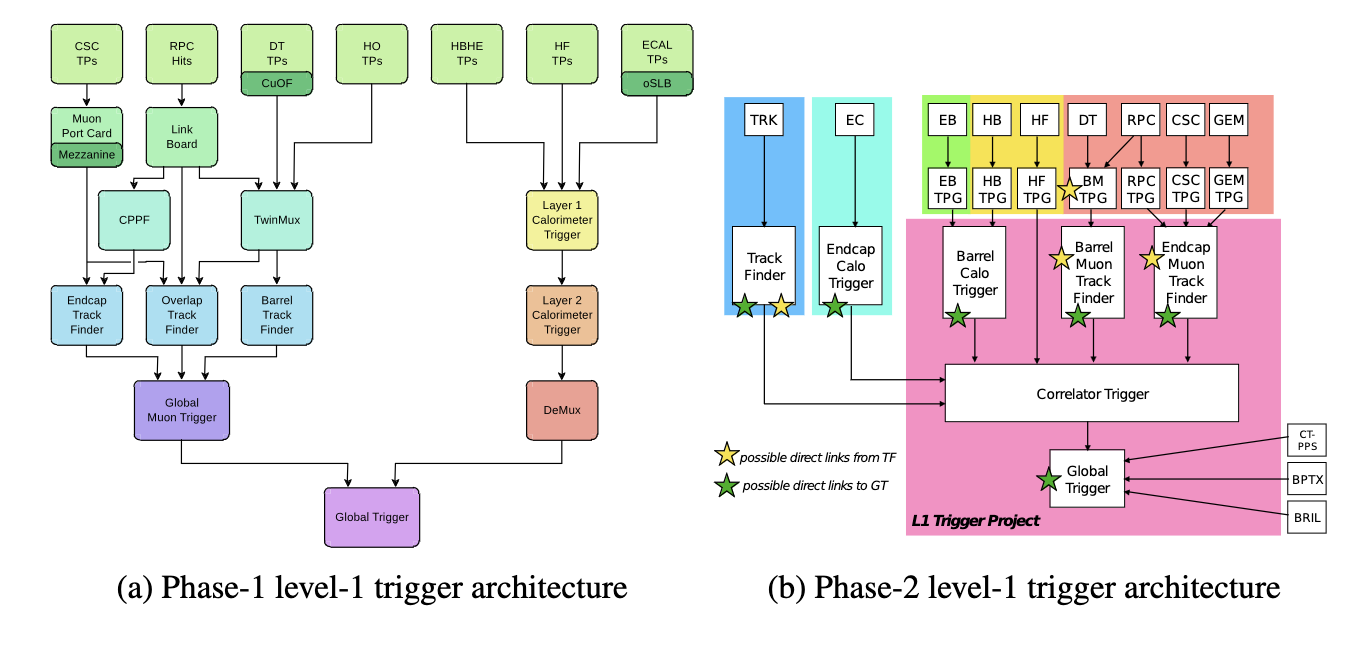
\includegraphics[width=0.7\linewidth]{images/cms/l1t-phase2.png}
    \caption{Overview of the Phase-1 (Run 2) and Phase-2 (Run 4) level-1 trigger architectures. In the former, inputs from the calorimeter and muon chamber are sent to the respective trigger subsystems, which are responsible for computing trigger objects. In the latter, three new systems are introduced: the endcap calorimeter trigger, responsible for processing data from HGCAL; the track finder, which reconstructs tracks in the tracker; the correlator trigger, which runs particle flow algorithms\cite{bologna2019overviewcms}.}
    \label{fig:cms-L1}
\end{figure}

In order to even maintain the current trigger performance in efficiency, resolution and background rejection the TDAQ system requires significant advancement. These performance improvements come jointly from the detector upgrades and their employment in reconstruction algorithms/trigger primitive decisions.
\par
In the upgraded L1 trigger\cite{bologna2019overviewcms} the maximum event rate is increased to $750$kHz from the previous $100$kHz with a new latency of $12.5${\textmu}s. L1 will now incorporate tracking inputs (for particles with $p_T$ exceeding a configurable threshold) in $|\eta|<2.4$. The track stubs will be filtered in an FPGA-based parallelized track-finding system. $3$ dimensional energy clusters from HGCAL will be included together with a full granularity readout of the barrel ECAL. The L1 trigger will have the capability to execute composite correlator trigger algorithms such as PF\cite{petrucciani2019particlecms} or Pile-Up-Per-Particle-Identification (PUPPI)\cite{kreis2018particlecms,bertolini2014puppi}.
\vspace{12pt}

The HLT in HL-LHC conditions will be required to manage a much higher event rate, more complex events and therefore a vast increase in computing requirements\cite{collaboration2021cmshlt}. The HLT will, as it does in Run 3, reduce the L1 event rate by a factor $100$; in the high-luminosity conditions this rate will be between $5$ and $7.5$kHz.
It is envisioned that $\sim 80\%$ of the computing workload will be ported to GPUs or other co-processors\cite{morovic2023cms}. The HLT will leverage the new HGCAL sub-detector and new tracker system, however these new sub-detectors are much more complex than their predecessors and the HLT will be required to have a throughput of $44$ Tb/s\cite{tomei2022hltcms}.






% \url{https://cds.cern.ch/record/2797771/files/CR2019_165.pdf}



\section{Use of real-time analysis for physics results}
\label{sec:RTA_physics}
%Caterina having a first go, but students will edit further during circulation period

In this section, we briefly outline the physics analyses that have been performed by ATLAS, CMS and LHCb using real-time analysis (RTA) in Run-1 and Run-2. 

%\textbf{Note: this section has not yet been reviewed by CMS SMARTHEP participants, please point out any inaccuracies during the comments period.}
%\subsection{CMS}

%From Patin: 

%Jet:
%Run1: https://cds.cern.ch/record/1461223, https://arxiv.org/abs/1604.08907
%Run2: https://arxiv.org/abs/1911.03761, https://arxiv.org/abs/1611.03568, https://arxiv.org/abs/1806.00843, https://arxiv.org/abs/1810.10092 
%Muon:
%Run2: https://arxiv.org/abs/2112.13769, https://arxiv.org/abs/1912.04776, https://cds.cern.ch/record/2851121, https://arxiv.org/abs/2305.04904

The \textit{data scouting} stream in CMS has been in place since the LHC Run-1 \cite{CMS-DP-2012-022}, and its first use in searches for dijet resonances is described in Ref. \cite{CMS-PAS-EXO-11-094}. 
RTA allows the reach of this search to be extended to resonances with masses of 600 GeV upwards, improving on the the standard data-taking analysis that would only be sensitive to resonances with masses of 1 TeV and above\footnote{Other techniques also exist beyond RTA to reach lower resonance masses, e.g. by triggering on initial state radiation or considering boosted jets that contain the resonance products.}. The same search has also been performed with the 8 and 13 TeV center-of-mass LHC datasets in Run-1 and Run-2, and described in Refs. \cite{CMS:2016ltu, CMS:2016gsl, CMS:2018mgb}, extending the Run-1 reach to 500 GeV resonance masses; a complementary search using a third jets for triggering reaches resonance masses of 350 GeV \cite{CMS:2019mcu}. ATLAS also searched for dijet resonances using the \textit{Trigger Level Analysis (TLA)} technique starting from Run-2, with sensitivity for resonances with masses as low as 450 GeV, as described in Ref. \cite{ATLAS:2018qto}. 

%CD: missing dijet+ISR? 

Searches for multijet resonances (new particles decaying in paired dijet and three jets each) are also using RTA, as shown in Ref. \cite{CMS:2018ikp}. RTA extends the reach of previous searches to the low mass region from 200 GeV down to 70 GeV for RPV squarks and gluinos. 

CMS also uses RTA in searches for dark photons and new long-lived particles decaying into muons using Run-2 data. Refs. \cite{CMS:2019buh, CMS:2023hwl} describe searches for dark photons decaying into dimuons that uses RTA in the 11.5-45 GeV mass range and between 1.1 and 7.9 GeV (excluding the 2.6 - 4.2 GeV window) respectively. In Ref. \cite{CMS:2021sch}, RTA enables access to the new phase space of low dimuon masses and non-zero displacement that would otherwise not be covered by standard searches.
The high event rate afforded by RTA also permitted the observation of the rare decay of the $\eta$ meson to four muons, described in Ref. \cite{CMS:2023thf}. 

%\subsection{LHCb}

In the LHCb context real-time analysis was motivated~\cite{Gligorov:2018fuk} by the size of the LHC production cross-section of hadrons containing a charm quark. Because this cross-section is so large, it is not possible to record all signal decays of charmed hadrons to permanent storage while keeping the full detector information for each event. For the same reason these decays must be fully reconstructed and selected in real-time, which means that the most accurate detector alignment and calibration must be used in the real-time processing to keep systematic uncertainties under control. This is particularly crucial since LHCb has a unique ability to probe $CP$ violation in charm hadrons to the $10^{-5}$ level or better, requiring a corresponding control of systematics. For this reason, LHCb implemented the full offline-quality reconstruction, alignment, and calibration~\cite{Dujany:2015lxd,Aaij:2016rxn,Borghi:2017hfp,LHCb:2018zdd,Aaij:2019uij} of the detector within its real-time processing (specifically the software trigger) during Run~2, and adopted real-time analysis as the baseline model~\cite{LHCbCollaboration:2319756} for the majority of the collaboration's physics programme from Run~3 onwards. Already during Run~2 almost all analyses of charm hadrons as well as certain searches for BSM states, most notably dark photons, were carried out using real-time analysis.
\section{Conclusion}

The trigger systems at the major LHC experiments have undergone a continuous evolution throughout their operation in Run~1 and Run~2. Significant upgrades have been implemented and proposed to address the challenges posed by the current Run~3 and future high luminosity conditions. The triggers now take advantage of modern hardware developments in the sub-detector readouts and novel data processing software including contemporary machine learning developments. The result today is a more robust, flexible and efficient trigger system, better able to accommodate future requirements.

In Run~3, the major LHC experiments leverage their experience from Run~1 and Run~2 to tackle increased data challenges. In particular, upgrades to these experiments and their respective trigger systems take advantage of recent advances in hardware technologies, with software frameworks redesigned to better capitalise on such upgrades. New and optimised software frameworks also provide implementations for faster and more capable algorithms for reconstruction, selection and data manipulation. Overall, this experience will be integrated into the plans for Run-4, also taking advantage of new detectors and new trigger hardware capabilities. 


%\section{Conclusions}
%If the document purpose calls for conclusions, this would be the place to put them.

\section*{Acknowledgements}
%This is important, as it acknowledges our funding. 
This work is part of the SMARTHEP network and it is funded by the European Union’s Horizon 2020 research and innovation programme, call H2020-MSCA-ITN-2020, under Grant Agreement n. 956086. 

\bibliography{references, references_intro, references_LHCb, references_ALICE, reference_ATLAS, references_CMS, references_RTA}
\bibliographystyle{JHEP}

\section*{Appendix}

\subsection{ATLAS detector}

The ATLAS detector\cite{ATLASMachine} is a general-purpose detector consisting of several sub detectors covering nearly all the area around the collision point. The detectors consist of the inner detector(ID), electromagnetic and hadronic calorimeters and a muon system. A small superconducting solenoid surrounds the inner detector with three large superconducting toroids(one around the barrel and two in the endcaps) around the calorimetry.

The inner detector surrounds the beam pipe, has a 2T axial magnetic field and measures momentum in the $|\eta| < 2.5$ region. The detector consists of three sub-detectors pixel, silicon microstrip and transition radiation trackers. The pixel tracker is situated closest to the beam pipe and is designed for a high-radiation environment. The highly granular detector makes on average 4 measurements per track. Following the pixel is the silicon microstrip detector which one average makes 4 measurements resulting in 4 space points. %Why?
The transition radiation tracker(TRT) surrounds the semiconductor detector in the barrel region(only barrel???) and consists of 4 mm drift straw tubes, generating trackick up to $|\eta| < 2.0 $. A track typically registers 36 hits per track in the TRT.

The calorimetry of ATLAS surrounds the solenoid and the ID with a coverage of $|\eta| < 4.9$. The electromagnetic calorimeter covers the barrel region($|\eta| < 1.475$) and the endcaps($1.375 < |\eta| < 3.2 $) with high-granularity lead/liquid-Argon(lAr) calorimetery. The hadronic section consists of tile calorimetry in the barrel and extended barrel regions($|\eta| < 1.7 $), the tile calorimetry use scintillating tiles as the active material and steel as the absorber. Additionally, the covered region is extended using an end-cap calorimeter covering $1.5 < |\eta| < 3.2 $ with lAr as the active material and copper absorbers. Finally, a dense forward calorimeter coveres the forward region inside the hadronic end-cap up to $|\eta| < 4.9 $.

The muon spectrometer covers the outermost parts of the ATLAS detector, the deflection of the muon tracks by the magnet system is use for the $p_T$ meaurements. The muon spectrometer consist of four sub-systems in three layers(cylindrical around beam axis in the barrel and perpendicular to the beam axis in the end-cap): Monitored Drift Tubes(MDT) and Cathode Strip Chambers(CSC) for precision tracking and Resistive Plate Chambers(RPC) and Thin Gap Chambers(TGC) for triggering.

\end{document}
